\documentclass[11pt,a4paper]{article}
\usepackage[UTF8,fontset=none]{ctex}
\usepackage[margin=2.5cm]{geometry}
\usepackage{hyperref}
\usepackage{longtable}
\usepackage{booktabs}
\usepackage{array}
\usepackage{enumitem}
\usepackage{titlesec}
\usepackage{graphicx}
\usepackage{algorithm}
\usepackage{algpseudocode}
\usepackage{amsmath}
\usepackage{amssymb}

\title{Meta-Encryptor Sealed 文件格式标准（中文草案）}
\author{YeeZ Tech}
\date{\today}

\setlist[itemize]{leftmargin=2em}
\setlist[enumerate]{leftmargin=2em}
\newcommand{\ttf}[1]{\texttt{\detokenize{#1}}}
% 排版约定：字段名用 \ttf{field_name}（勿在参数内写 \_）；算法变量用 $H_0$ 等；
% 多项并列写在同一 enumerate 项时，用嵌套 itemize 拆开，勿用长逗号串。
\newcommand{\rollhash}{\mbox{滚动摘要}}
\newcommand{\secref}[1]{第~\ref{#1}~节}
\XeTeXlinebreaklocale "zh"
\XeTeXlinebreakskip = 0pt plus 0.15em minus 0.05em
\setCJKmainfont{PingFang SC}
\setCJKsansfont{PingFang SC}
\setCJKmonofont{PingFang SC}

% 减轻正文过长行导致的 Overfull \hbox（中文技术长句、交叉引用）
\setlength{\emergencystretch}{2.5em}
\setlength{\tolerance}{2000}
\hbadness=10000
\sloppy

\begin{document}
\maketitle
\section*{文档元数据}
\begin{longtable}{>{\raggedright\arraybackslash}p{3.2cm} >{\raggedright\arraybackslash}p{10.0cm}}
  \toprule
  字段     & 内容                                      \\
  \midrule
  \endhead
  文档标识   & \ttf{YEEZ-SEALED-FORMAT-ZH}             \\
  文档状态   & Draft（草案）                               \\
  文档版本   & v0.2.0（草案）                              \\
  发布日期   & \today                                  \\
  语言     & 中文（规范性文本）                               \\
  适用范围   & Meta-Encryptor 生态下 \ttf{.sealed} 文件读写实现 \\
  解释优先级  & 本标准正文优先于示例代码；示例仅作实现参考                   \\
  变更记录策略 & 仅在“对外发布版本”时更新变更记录；日常本地迭代与排版修订不单独记入版本历史  \\
  \bottomrule
\end{longtable}

\section*{发布级变更记录}
\begin{longtable}{>{\raggedright\arraybackslash}p{2.2cm} >{\raggedright\arraybackslash}p{2.8cm} >{\raggedright\arraybackslash}p{6.8cm}}
  \toprule
  版本           & 日期     & 说明                                  \\
  \midrule
  \endhead
  \ttf{v0.1.0} & ---  & 首个公开草案：定义文件结构、密码学规范、封装/解封流程、错误码与附录。 \\
  \ttf{v0.2.0} & \today & Header 80 字节；以 Item 为最小单元（取消输入单元/批包/批刷写阈值）；载荷由集成层定义；第 9 章目录树明文格式、第 10 章多文件封装与解封（框架）。 \\
  \bottomrule
\end{longtable}

\tableofcontents
\newpage

\section{引言}
\subsection{目的}
本标准用于定义 \texttt{.sealed} 文件格式的二进制结构、加密语义、封装与解封流程、兼容性规则与一致性要求，确保不同实现之间的互操作性与可验证性。

\subsection{范围}
本标准适用于使用 Meta-Encryptor 生态读写 \texttt{.sealed} 文件的实现，包括但不限于 Node.js 与浏览器环境实现。本文档不限定上层业务协议。
第~\ref{sec:seal-chapter}、\ref{sec:unseal-chapter} 章规定\textbf{按序 Item 载荷}的封装与解封；第~\ref{sec:directory-tree-chapter} 章规定目录树明文布局与解析；第~\ref{sec:multi-file-chapter} 章描述多文件封装与整包解封（参考流程）。

\subsection{读者对象}
本标准面向以下读者：
\begin{itemize}
  \item 文件格式实现者；
  \item 安全审计人员；
  \item 平台集成与运维工程师；
  \item 隐私计算数据处理链路设计人员。
\end{itemize}

\subsection{一致性语言}
本文档使用 RFC 2119 含义的以下术语：
\begin{itemize}
  \item \textbf{必须（MUST）}：对文件布局、字段取值、可验证一致性及失败语义的绝对要求；
  \item \textbf{应当（SHOULD）}：推荐要求，除非有充分理由；
  \item \textbf{可以（MAY）}：可选行为。
\end{itemize}

\textbf{适用范围：} 第~\ref{sec:format-chapter} 章、第~\ref{sec:crypto-chapter} 章，以及各章中对上述内容的直接引用，使用 MUST/SHOULD/MAY 表述\textbf{格式与校验}义务。
第~\ref{sec:seal-chapter}、\ref{sec:unseal-chapter} 章给出\textbf{参考封装/解封流程}，描述 Meta-Encryptor 生态常用的实现顺序；除明确援引格式或校验条款外，流程步骤本身不以 MUST 约束具体算法或数据结构（如读指针、队列）。

\section{术语与记号}
\subsection{术语}
\begin{itemize}
  \item \textbf{Item}：\texttt{.sealed} 内容区中\textbf{最小不可分}单元；每条 Item 对应一段由集成层定义的 \textbf{Item 载荷}（\ttf{item_payload}），经加密后写入内容区（见第~\ref{sec:content-region}、\ref{sec:item-payload-norms} 节）；
  \item \textbf{Block}：由若干 Item 组成的逻辑分组，并在元信息区有对应索引项；
  \item \textbf{Header}：文件尾部固定 80 字节头结构（含目录树 Item 定位字段，见第~\ref{sec:header-region} 节）；
  \item \textbf{Item 载荷流}：封装侧按序提交、解封侧按序还原的 \ttf{item_payload} 序列；每个逻辑文件（含目录树文件）经集成层映射为一条或多条 Item 载荷后，走第~\ref{sec:seal-chapter} 章同一管道；
  \item \textbf{Block Info}：描述单个 Block 的 32 字节索引结构；\textbf{Block Infos 区}为由若干条 Block Info 顺序拼接而成的索引区域；
  \item \textbf{Data Hash}：Header 字段 \ttf{data_hash} 所承载的摘要；对全部 Item 的 \ttf{item_payload} 按 Item 全局顺序滚动计算，见第~\ref{sec:rolling-hash} 节；
  \item \textbf{Item 载荷}：本条 Item 在密码学模块与滚动摘要边界上的输入，记为 \ttf{item_payload}；类型为变长字节串（\texttt{VARBYTES}，见第~\ref{sec:item-payload-norms} 节），\textbf{不是} Unicode 字符串、数值或其它结构化类型；一条 Item 对应一条 \ttf{item_payload}；
  \item \textbf{业务载荷}：宿主侧的 \ttf{payload}（业务对象）；进入 \ttf{item_payload} 前的编码、切分由集成层完成，不属于 \texttt{.sealed} 文件布局；
  \item \textbf{Block 内 Item 数上限} \ttf{N_block}：封装实现参数，限定单个 Block 所含 Item 条数的上界；划分规则见第~\ref{sec:block-split} 节；与 Block Info 字段的对应见第~\ref{sec:block-meta-fields} 节；
  \item \textbf{逻辑文件}：多文件场景下的一份业务侧文件，密封前由集成层映射为一条或多条 \ttf{item_payload}；解封后由目录树索引（见第~\ref{sec:directory-tree-chapter} 章）或按 Item 序输出还原；
  \item \textbf{目录（树）文件}：描述密封包内逻辑文件索引与层级的明文布局；密封时与其它逻辑文件相同，经 Item 载荷写入内容区；Header.\ttf{tree_item_index}、\ttf{tree_item_number} 指向其 Item 范围（见第~\ref{sec:header-region} 节）。
\end{itemize}

\subsection{数据类型}
\begin{itemize}
  \item \texttt{BYTE}：8 位无符号整数；
  \item \texttt{UINT32}：32 位无符号整数；
  \item \texttt{UINT64}：64 位无符号整数；
  \item \texttt{BYTESTRING[n]}：长度为 \texttt{n} 的字节串；
  \item \texttt{VARBYTES}：变长字节串（长度由外层字段定义）。
\end{itemize}

\subsection{字节序}
除非另有说明，多字节整数均使用\textbf{小端序（Little Endian）}。

\subsection{布局示意图中的 \texttt{B} 与 \texttt{b}}\label{sec:layout-notation-units}
本章及后文用方括号示意字段顺序时，括号内单位约定如下：
\begin{itemize}
  \item \texttt{B}（大写）：\textbf{字节}（byte），表示该段占用的字节长度，如 \texttt{(8B)} 为 8 字节；
  \item \texttt{b}（小写）：\textbf{比特}（bit），表示该段占用的比特位数，用于单个整数类型内的按位打包字段，如 \texttt{(4b)} 为 4 比特；同一整数内多段按位字段与底层类型的字节序一致，\textbf{低位比特先行}（见第~\ref{sec:tree-child} 节 \ttf{child}）。
\end{itemize}
未标注 \texttt{B} 或 \texttt{b} 的长度说明，以对应小节的字段表为准。

\section{设计目标与安全模型}
\subsection{设计目标}
\begin{itemize}
  \item 提供面向隐私计算链路的数据封装格式；
  \item 支持流式封装与流式解封；
  \item 支持断点续传场景下的一致性恢复；
  \item 支持跨运行时（Node.js / Browser）一致解封。
\end{itemize}

\subsection{安全属性}
\begin{itemize}
  \item 机密性：明文对未授权方不可见；
  \item 完整性：篡改应可被检测；
  \item 认证性：每个 Item 具备认证加密保护。
\end{itemize}

\subsection{非目标}
\begin{itemize}
  \item 本标准不定义业务语义级字段；
  \item 本标准不定义应用层权限模型；
  \item 本标准不保证无索引情况下的记录级随机查询性能。
\end{itemize}

\section{文件格式总览}
\subsection{高层布局}
\texttt{.sealed} 文件采用“数据在前、元信息在后”的尾部头设计。文件按字节从前到后布局如下：
\begin{center}
  \texttt{[Content Region][Block Infos][Header(80B)]}
\end{center}
\begin{itemize}
  \item \ttf{Content Region}：密文内容区，由若干 Item 顺序拼接组成；各 Item（含目录树对应 Item）的加密形态一致。内容区按块组织，详见第~\ref{sec:content-region} 节；
  \item \ttf{Block Infos}：块索引区，由若干 Block Info 顺序拼接而成；每条 Block Info 固定 32 字节，条数由 Header 给出，详见第~\ref{sec:block-infos} 节；
  \item \ttf{Header}：固定 80 字节，位于文件末尾，包含魔数、版本、计数、摘要及目录树 Item 定位字段，详见第~\ref{sec:header-region} 节；
\end{itemize}
该布局允许写入端在不知道最终计数的情况下先持续写入内容，再在结束时一次性写入索引和 Header。

\subsection{读取模型}\label{sec:read-model}
由于 Header 位于尾部，标准定义两种等价读取模型：
\begin{itemize}
  \item \textbf{尾读模型}：读取器先从文件末尾读取 80B Header（字段布局见第~\ref{sec:header-region} 节），再按 Header.\ttf{block_number} 读取 Block Infos 区，再读取内容区；
  \item \textbf{逻辑前置模型}：中间层先尾读 Header，并在解封管道中将 Header 逻辑前置，再按顺序喂入内容区数据。
\end{itemize}
两种模型 MUST 产出一致的解析结果。

\subsection{区域长度计算}\label{sec:region-length}
本小节使用的符号先定义如下：
\begin{itemize}
  \item \ttf{block_number}：\ttf{Header} 结构中的字段，表示 Block Info 条目数量（类型为 \ttf{UINT64(LE)}）；
  \item \ttf{N}：\ttf{block_number} 的记号化表示，即 \ttf{N = block_number}；
  \item \ttf{file_size}：单个 \texttt{.sealed} 文件的总字节数；由打开文件、对象大小或传输层长度字段等在\textbf{读取 Header 之前}由实现获知，不得通过解析 Header 反推。
  \item \ttf{header_size}：Header 区总长度（单位：字节）；
  \item \ttf{block_infos_size}：Block Infos 区总长度（单位：字节）；
  \item \ttf{content_size}：Content Region 区总长度（单位：字节）。
\end{itemize}

给定文件总长度 \ttf{file_size}，则：
\begin{itemize}
  \item \ttf{header_size = 80}
  \item \ttf{block_infos_size = 32 * N}
  \item \ttf{content_size} $=$ \ttf{file_size} $-$ \ttf{header_size} $-$ \ttf{block_infos_size}
\end{itemize}
实现 MUST 校验 \ttf{content_size > 0}。若不满足，MUST 视为格式错误。

\section{二进制格式规范}\label{sec:format-chapter}
\subsection{规范约定}
\begin{itemize}
  \item 除特别说明外，整数类型均为无符号；
  \item 除特别说明外，所有多字节整数均为小端序（LE）；
  \item 偏移均以“所在结构体起始地址”为基准；
  \item 本章字段名使用实现同名风格（如下划线命名）以便互操作。
\end{itemize}

\subsection{Header 区}\label{sec:header-region}
Header 区位于文件末尾，长度固定为 80 字节。本区由单个 Header 记录构成，保存格式识别、版本、块与 Item 计数、数据摘要，以及目录树 Item 在内容区中的定位信息。

\textbf{说明：} 目录（树）文件与其它逻辑文件在 Content Region 中均为普通 Item，差异仅体现在明文语义及 Header 对目录树 Item 下标的标注；目录明文布局见第~\ref{sec:directory-tree-chapter} 章，多文件封装与整包解封见第~\ref{sec:multi-file-chapter} 章。

\subsubsection{Header 记录（80 字节）}
Header 记录占用 80 字节，字段布局如下：
\begin{longtable}{>{\raggedright\arraybackslash}p{3.4cm} >{\raggedright\arraybackslash}p{1.2cm} >{\raggedright\arraybackslash}p{1.2cm} >{\raggedright\arraybackslash}p{6.6cm}}
  \toprule
  字段名                  & 偏移 & 长度 & 说明                   \\
  \midrule
  \endhead
  \ttf{magic_number}      & 0  & 8  & 文件魔数（\ttf{BYTESTRING[8]}）  \\
  \ttf{version_number}    & 8  & 8  & 格式版本（\ttf{UINT64, LE}）     \\
  \ttf{block_number}      & 16 & 8  & Block 数量（\ttf{UINT64, LE}） \\
  \ttf{item_number}       & 24 & 8  & Item 总数量（\ttf{UINT64, LE}）  \\
  \ttf{data_hash}          & 32 & 32 & 数据摘要（\ttf{BYTESTRING[32]}） \\
  \ttf{tree_item_index}   & 64 & 8  & 目录树起始 Item 下标（\ttf{UINT64, LE}，含） \\
  \ttf{tree_item_number}  & 72 & 8  & 目录树占用 Item 条数（\ttf{UINT64, LE}） \\
  \bottomrule
\end{longtable}
\textbf{字段语义：}
\begin{itemize}
  \item \ttf{magic_number}：文件类型标识（\ttf{BYTESTRING[8]}）；
  \item \ttf{version_number}：格式版本；
  \item \ttf{block_number}：Block Info 条目数量；维护规则见第~\ref{sec:block-meta} 节；
  \item \ttf{item_number}：内容区 Item 总数量（见第~\ref{sec:content-region} 节）；每写出一条 Item 递增，见第~\ref{sec:item-generation} 节；
  \item \ttf{data_hash}：对全部 Item 的 \ttf{item_payload}（按 Item 全局顺序）滚动计算得到的最终摘要（\ttf{BYTESTRING[32]}）。
        累计规则见第~\ref{sec:rolling-hash} 节；Item 载荷要求见第~\ref{sec:item-payload-norms} 节；
        算法与写入见第~\ref{sec:rolling-hash}、\ref{sec:seal-finalize} 节；
        解封校验见第~\ref{sec:integrity-check} 节。
  \item \ttf{tree_item_index}、\ttf{tree_item_number}：自 \ttf{tree_item_index} 起（含）连续 \ttf{tree_item_number} 条 Item 为目录树密文；
        目录树明文布局见第~\ref{sec:directory-tree-chapter} 章；\ttf{tree_item_number} 为 0 时表示无目录树（见第~\ref{sec:directory-tree-no-tree}、\ref{sec:multi-file-no-tree} 节）。
\end{itemize}

\subsubsection{Header 识别与版本兼容规则}\label{sec:header-compat}
本小节统一约束 \ttf{magic_number} 与 \ttf{version_number} 的识别、校验与版本演进策略：
\begin{itemize}
  \item \textbf{文件}：指单个 \ttf{.sealed} 文件实例；
  \item \textbf{实现}：指遵循本标准的读写器（Writer/Reader）；
  \item \textbf{未来版本}：指 \ttf{version_number} 高于当前版本的格式版本。
\end{itemize}
\begin{itemize}
  \item 每个 \ttf{.sealed} 文件 MUST 在 Header 中携带 \ttf{version_number}；
  \item \textbf{文件识别}：\ttf{magic_number} MUST 等于约定魔数；
  \item \textbf{版本识别}：\ttf{version_number} MUST 位于实现声明的支持范围内；
  \item 读取实现 MUST 在进入内容解析前完成上述检查；
  \item 任一检查失败时，读取器 MUST 拒绝继续解析。
  \item 新版本在可行时 SHOULD 保持向后兼容；若无法兼容，MUST 提供迁移或拒绝策略说明。
\end{itemize}

\subsubsection{当前版本 Header 字段约定值}
当前版本（\ttf{version_number = 2}）的 Header 字段约定值如下：
\begin{itemize}
  \item \ttf{magic_number = 1fe2ef7f3ed18847}
\end{itemize}
若后续版本调整上述字段取值或字段语义，\ttf{version_number} MUST 递增并提供兼容说明。

\subsection{Block Infos 区}\label{sec:block-infos}
Block Infos 区位于 Content Region 与尾部 Header 之间，总长度 \ttf{block_infos_size}
及其在文件中的起止位置由第~\ref{sec:region-length} 节给出。

本区由 \ttf{block_number} 条 Block Info 顺序拼接而成。本文所称单条 \textbf{Block Info}，即长度为 32 字节的索引记录；\textbf{Block Infos 区}即上述全部 Block Info 按序拼接形成的区域。本区总长度为 \ttf{32 * block_number}。第 \ttf{i} 条 Block Info（\ttf{i} 自 0 起）在本区内的字节偏移为 \ttf{32 * i}。

\subsubsection{Block Info 记录（每项 32 字节）}
每条 Block Info 对应 Content Region 中的一个 Block：在 Item 下标维度标出该 Block 覆盖的 Item 范围，在内容区字节偏移维度标出上述 Item 序列所占用的字节范围。两条范围彼此对应。字段布局如下：
\begin{longtable}{>{\raggedright\arraybackslash}p{3.4cm} >{\raggedright\arraybackslash}p{1.2cm} >{\raggedright\arraybackslash}p{1.2cm} >{\raggedright\arraybackslash}p{6.8cm}}
  \toprule
  字段名                    & 偏移 & 长度 & 说明                      \\
  \midrule
  \endhead
  \ttf{start_item_index} & 0  & 8  & 起始 Item 下标（含）           \\
  \ttf{end_item_index}   & 8  & 8  & 结束 Item 下标（不含）          \\
  \ttf{start_file_pos}   & 16 & 8  & 内容区内起始字节偏移（非源明文文件偏移）    \\
  \ttf{end_file_pos}     & 24 & 8  & 内容区内结束字节偏移（半开，非源明文文件偏移） \\
  \bottomrule
\end{longtable}
\textbf{字段语义：}
\begin{itemize}
  \item \ttf{start_item_index}、\ttf{end_item_index}：该 Block 内 Item 的下标半开区间 \ttf{[start, end)}，下标从 0 起计；
  \item \ttf{start_file_pos}、\ttf{end_file_pos}：本 Block 在 \texttt{.sealed} 文件 Content Region 内占据的字节半开区间 \ttf{[start, end)}，偏移以内容区首字节为 \texttt{0}；\textbf{不}表示业务侧源文件内偏移（见第~\ref{sec:block-meta-fields} 节）。
\end{itemize}
全体 Block Info 共同构成 Content Region 的块级索引：
\begin{itemize}
  \item Item 下标维度：各 Block 的 \ttf{start_item_index}、\ttf{end_item_index} 以半开区间无空隙、无重叠地划分
        \ttf{[0, item_number)}；
  \item 内容区字节维度：各 Block 的 \ttf{start_file_pos}、\ttf{end_file_pos} 以内容区起点为 0，同样无隙、无重叠地划分 \ttf{[0, content_size)}。
\end{itemize}

\subsection{Content Region 区}\label{sec:content-region}
Content Region 区位于文件最前部，在 Block Infos 区与 Header 区之前；总长度 \ttf{content_size}
及其在文件中的起止位置由第~\ref{sec:region-length} 节给出。

本区由 \ttf{item_number} 条 Item 顺序拼接而成。本文所称单条 \textbf{Item}，即内容区\textbf{最小不可分}单元，对应一条 \ttf{item_payload}（见第~\ref{sec:item-payload-norms} 节）；\textbf{Content Region 区}即上述全部 Item 按序拼接形成的区域。内容区按块组织，每块由若干连续的 Item 组成。各条 Item 长度随密文载荷变化，Item 之间无固定步长。

\subsubsection{Item 记录}\label{sec:item-record}
每条 Item 由前置长度字段与密文载荷顺序组成，按字节从前到后布局如下：
\begin{center}
  \texttt{[item\_size (8B)][cipher\_payload (item\_size B)]}
\end{center}
完整展开（含 \texttt{cipher\_payload} 内部字段）为：
\begin{center}
  \small
  \texttt{[item\_size (8B)][encrypted\_data (变长)][iv (12B)][ephemeral\_public\_key (64B)][gcm\_tag (16B)]}
\end{center}
字段说明：
\begin{enumerate}
  \item \texttt{item\_size}：8 字节无符号整数（LE）；
  \item \texttt{cipher\_payload}：长度为 \texttt{item\_size} 的字节串。
\end{enumerate}
\textbf{注意：} \ttf{item_size} 仅描述当前 Item 的密文载荷长度，不包含其自身 8 字节长度字段；其取值范围由 \ttf{UINT64(LE)} 确定，\ttf{cipher_payload} 的字节长度 MUST 等于 \ttf{item_size}，且 MUST NOT 超过 \ttf{UINT64} 可表示的最大值。

\subsubsection{\texttt{cipher\_payload} 内部结构}\label{sec:cipher-payload-layout}
\ttf{cipher_payload} 长度为 \ttf{item_size}，自其起始偏移 0 起按字节从前到后布局如下：
\begin{center}
  \texttt{[encrypted\_data (变长)][iv (12B)][ephemeral\_public\_key (64B)][gcm\_tag (16B)]}
\end{center}
后三段长度在当前版本固定，\ttf{encrypted_data} 变长；四段顺序拼接，字段说明如下：
\begin{enumerate}
  \item \texttt{encrypted\_data}（变长）；
  \item \texttt{iv}（12B）；
  \item \texttt{ephemeral\_public\_key}（64B）；
  \item \texttt{gcm\_tag}（16B）。
\end{enumerate}
\textbf{字段语义：}
\begin{itemize}
  \item \ttf{encrypted_data}：\ttf{AES-128-GCM} 密文；解密并解码后得到本条 Item 的 \ttf{item_payload}（见第~\ref{sec:item-payload-boundary}、\ref{sec:crypto-chapter} 节）；
  \item \ttf{iv}：本条 Item 的 \ttf{AES-128-GCM} Nonce（常称 IV）；供加解密双方标识本次独立 GCM 运算，避免同一密钥下因 Nonce 复用而产出相同密文。长度固定 12 字节，取值由安全随机源逐 Item 生成，见第~\ref{sec:randomness} 节；
  \item \ttf{ephemeral_public_key}：本 Item 临时密钥对的公钥；采用椭圆曲线型号 \texttt{secp256k1} 的未压缩公钥，去掉首字节 \texttt{0x04} 后保留 \texttt{x||y}，长度固定 64 字节；
  \item \ttf{gcm_tag}：\ttf{AES-128-GCM} 认证标签；长度固定 16 字节，由 GCM 运算得到。
\end{itemize}
\textbf{当前版本固定长度与偏移：}
\begin{itemize}
  \item \ttf{encrypted_data_len = item_size - 12 - 64 - 16}；
  \item \ttf{iv} 起始于 \ttf{encrypted_data_len}，长度 12 字节；
  \item \ttf{ephemeral_public_key} 起始于 \ttf{encrypted_data_len + 12}，长度 64 字节；
  \item \ttf{gcm_tag} 起始于 \ttf{encrypted_data_len + 76}，长度 16 字节；
  \item 若 \ttf{encrypted_data_len < 0}，读取器 MUST 返回格式错误。
\end{itemize}
上述 12、64、16 字节为当前版本规定的尾字段长度；\ttf{iv}、\ttf{ephemeral_public_key}、\ttf{gcm_tag} 与 \ttf{encrypted_data} 的字节值逐 Item 变化，除长度外无固定取值。Item 密文封装使用的前缀字节为 \texttt{0x02}，见第~\ref{sec:ref-derive-params} 节。

\subsection{Item 载荷与加密边界}\label{sec:item-payload-boundary}
内容区每条 Item 在\textbf{内容加密模块入口}（第~\ref{sec:content-encryption} 节）处的输入为一条 \ttf{item_payload}；其基本类型与语义约束见第~\ref{sec:item-payload-norms} 节。\textbf{一条 Item 对应一条} \ttf{item_payload}。

当前版本（\ttf{version_number = 2}）内容加密模块的具体运算见第~\ref{sec:content-encryption} 节；\texttt{.sealed} 文件内\textbf{不}另设批包容器或 \ttf{package_id} 记录层。

\subsection{约束与限制}
\begin{itemize}
  \item Header 固定长度为 80 字节；
  \item Block Info 固定长度为 32 字节；
  \item Item 数量与 Block 数量 MUST 与实际内容一致；
  \item 超出实现上限时 MUST 返回错误。
\end{itemize}

\subsection{规范性解析流程}
实现方在读取 \texttt{.sealed} 时 MUST 按以下顺序执行：
\begin{enumerate}
  \item 从文件末尾读取 80 字节 Header；
  \item 校验 \ttf{magic_number} 和 \ttf{version_number}；
  \item 基于 \ttf{block_number} 计算并定位 Block Infos 区；
  \item 校验 \ttf{content_size} 为正且区域不重叠；
  \item 顺序解析内容区 Item：先读 \ttf{item_size}，再读 \ttf{cipher_payload}；
  \item 每个 Item 执行长度合法性检查和密码学认证检查；
  \item 当解析 Item 数量达到 \ttf{item_number} 时结束并进入完整性校验阶段。
\end{enumerate}
全量顺序解封时，上述 MUST 条款与第~\ref{sec:unseal-chapter} 章参考流程及第~\ref{sec:unseal-total-algorithm} 节应对齐；块级随机访问见第~\ref{sec:random-access-chapter} 章。

\subsection{规范性校验规则}
\begin{itemize}
  \item \textbf{计数校验}：实际解析 Item 数 MUST 等于 \ttf{item_number}；
  \item \textbf{区间校验}：最后一个 Block 的 \ttf{end_item_index} SHOULD 等于 \ttf{item_number}（Block Info 语义见第~\ref{sec:block-meta-fields} 节）；
  \item \textbf{边界校验}：任一 \ttf{start > end} 或越界偏移 MUST 判为错误；
  \item \textbf{摘要校验}：实现 SHOULD 按第~\ref{sec:rolling-hash} 节重算摘要并比对 Header.\ttf{data_hash}，不一致 MUST 报错（亦见第~\ref{sec:integrity-check} 节）；
  \item \textbf{版本校验}：未知版本 MAY 拒绝处理；若处理 MUST 在实现文档中声明兼容边界。
\end{itemize}

\section{密码学规范}\label{sec:crypto-chapter}
本章规定 \ttf{version_number = 2} 下 Item 密文载荷的密码学处理要求。
第~\ref{sec:key-derivation}、\ref{sec:aes-gcm}、\ref{sec:content-encryption} 节按\textbf{模块}给出输入与输出；其余小节为概念、常量或约束说明。
符号 \ttf{item_payload} 含义见第 2 章；与 GCM 的编码边界见第~\ref{sec:item-payload-boundary} 节。

\subsection{曲线与密钥}\label{sec:curve-keys}
本小节规定逐条 Item 协商对称密钥所需的曲线型号与密钥材料。

Item 的 \ttf{encrypted_data} 由第~\ref{sec:aes-gcm} 节规定的 \texttt{AES-128-GCM}
保护。对称密钥不由接收方长期公钥直接充当，而是经临时密钥对与 ECDH 得到共享秘密，再经第~\ref{sec:key-derivation} 节派生
\ttf{session_key}。

\begin{itemize}
  \item \textbf{椭圆曲线}：\texttt{secp256k1}；
  \item \textbf{临时密钥对}：封装每条 Item 时 MUST 新生成（公钥写入 \ttf{ephemeral_public_key}）；不同 Item MUST 彼此独立；
  \item \textbf{ECDH}：封装侧以「本条 Item 临时私钥 + 接收方长期公钥」运算；解封侧以「接收方长期私钥 + \ttf{ephemeral_public_key}」运算；双方在曲线与格式一致时得到同一曲线点，再经第~\ref{sec:key-derivation} 节派生 \ttf{session_key}；
  \item \textbf{下游}：\ttf{session_key} 在第~\ref{sec:content-encryption}、\ref{sec:decrypt-crypto} 节\textbf{模块内部}使用，不对外作为独立调用接口。
\end{itemize}

\textbf{长期密钥与临时公钥格式：}
\begin{itemize}
  \item \textbf{长期公钥、长期私钥}：\texttt{.sealed} 文件内 \textbf{不} 保存接收方的长期公钥或私钥。封装时，写入端 MUST 在应用层向加密模块提供接收方长期公钥；解封时，读取端 MUST 在应用层提供对应的长期私钥。当前参考实现中，二者均以十六进制字符串传入：私钥 32 字节（64 个十六进制字符），公钥 64 字节 \texttt{x||y}（128 个十六进制字符，未压缩公钥去掉首字节 \texttt{0x04}）；模块内部再解码为曲线点参与 ECDH。
  \item \ttf{ephemeral_public_key}：\textbf{写入} \texttt{.sealed} 文件，为每条 Item 的临时公钥；64 字节 \texttt{x||y}，格式与长期公钥相同；参与 ECDH 时 MUST 在首部补回 \texttt{0x04}。
\end{itemize}

\subsection{密钥派生}\label{sec:key-derivation}
本小节规定\textbf{密钥派生}模块：将 ECDH 共享秘密转换为本条 Item 的 GCM 会话密钥 \ttf{session_key}。

\textbf{输入（来源）：}
\begin{itemize}
  \item \textbf{ECDH 所用密钥对}（运算规则见第~\ref{sec:curve-keys} 节）：封装侧为「本条 Item 临时私钥 + 接收方长期公钥」；解封侧为「接收方长期私钥 + \ttf{cipher_payload} 中的 \ttf{ephemeral_public_key}」；
  \item \ttf{cmac_key}、\ttf{derivation_buffer} 布局常量：见第~\ref{sec:ref-derive-params} 节。
\end{itemize}

\textbf{输出：}
\begin{itemize}
  \item \ttf{session_key}：16 字节，供第~\ref{sec:aes-gcm}、\ref{sec:content-encryption}、\ref{sec:decrypt-crypto} 节使用。
\end{itemize}

\subsubsection{ECDH 共享秘密}\label{sec:ecdh-shared-secret}
ECDH（Elliptic Curve Diffie-Hellman）是一类椭圆曲线密钥协商方法，可参照 SEC 1 的 ECDH 原语或 NIST SP
800-56A 中的 ECC CDH 密钥协商术语理解：一方使用自己的私钥与对方公钥运算，双方在参数一致时得到同一曲线点。当前版本的 ECDH 在
\texttt{secp256k1} 上完成，并将该曲线点按下述规则转换为 32 字节共享秘密 \ttf{shared_key}（与参考实现一致）：
\begin{itemize}
  \item 设 ECDH 结果为曲线点坐标 \texttt{(x, y)}，各 32 字节；
  \item 构造 33 字节缓冲区：首字节为 \texttt{0x02}（\texttt{y} 最低位为 0）或 \texttt{0x03}（\texttt{y} 最低位为 1），后接 \texttt{x}；
  \item \ttf{shared_key = SHA256(上述 33 字节)}。
\end{itemize}

\subsubsection{CMAC 派生会话密钥}\label{sec:cmac-session-key}
CMAC（Cipher-based Message Authentication Code）是一类基于分组密码的消息认证码，可参照 NIST SP
800-38B 中的 CMAC 模式理解；AES-CMAC 的具体算法也可参照 RFC 4493。国密算法体系中可类比以 SM4 等分组密码为底层算法的
CMAC 类用法，但当前版本固定使用 AES-CMAC，不引入 SM4 参数。

本标准将 \ttf{AES_CMAC(K, M)} 视为确定性函数：输入 16 字节密钥 \ttf{K} 与变长消息 \ttf{M}，输出 16 字节认证标签。当前版本不直接使用该标签做外部认证，而是将 AES-CMAC 用作密钥派生步骤。会话密钥由两步 AES-CMAC（128 位密钥、128 位标签）派生：
\begin{enumerate}
  \item \ttf{key_derive_key = AES_CMAC(cmac_key, shared_key)}，输出 16 字节；
  \item \ttf{session_key = AES_CMAC(key_derive_key, derivation_buffer)}，输出 16 字节，即本条 Item 的 \texttt{AES-128-GCM} 会话密钥。
\end{enumerate}

\textbf{\ttf{derivation_buffer} 布局（当前版本，共 25 字节）：}
\begin{center}
  \small
  \begin{tabular}{>{\raggedright\arraybackslash}p{1.8cm} >{\raggedright\arraybackslash}p{1.2cm} >{\raggedright\arraybackslash}p{8.8cm}}
    \toprule
    偏移 & 长度 & 内容                                           \\
    \midrule
    0  & 1  & 固定值 \texttt{0x01}                            \\
    1  & 21 & 域分离字符串 \texttt{tech.yeez.key.manager}（UTF-8） \\
    22 & 1  & 固定值 \texttt{0x00}                            \\
    23 & 1  & 固定值 \texttt{0x80}                            \\
    24 & 1  & 固定值 \texttt{0x00}                            \\
    \bottomrule
  \end{tabular}
\end{center}

\subsection{参考派生参数（当前版本）}\label{sec:ref-derive-params}
为保证互操作，当前版本 (\ttf{version_number = 2}) 采用下列固定参数（字符串均为 UTF-8，\textbf{无}换行符、\textbf{无} BOM）：
\begin{itemize}
  \item \ttf{cmac_key}（16 字节）：
        \begin{itemize}
          \item 字符串形式：\texttt{yeez.tech.stbox} 后接 1 字节 \texttt{0x00}（共 16 字节，\textbf{不}含额外换行或第二处 NUL）；
          \item 十六进制：\texttt{7965657a2e746563682e7374626f7800}。
        \end{itemize}
  \item 域分离字符串（21 字节）：
        \begin{itemize}
          \item 字符串形式：\texttt{tech.yeez.key.manager}（恰好 21 个 UTF-8 字节，\textbf{无}结尾 \texttt{0x00}、\textbf{无}换行）；
          \item 十六进制：\texttt{746563682e7965657a2e6b65792e6d616e61676572}。
        \end{itemize}
  \item 该字符串用于第~\ref{sec:cmac-session-key} 节 \ttf{derivation_buffer}（偏移 1 起 21 字节）及下文 GCM \ttf{AAD}（偏移 0 起 21 字节）；
  \item Item 载荷加密前缀字节：\texttt{0x02}（写入 AAD 偏移 24 处）；
  \item GCM \ttf{AAD} 容器长度：64 字节。
\end{itemize}

\ttf{AAD}（Additional Authenticated Data，附加认证数据）是不加密但参与认证的上下文字节串。GCM 会把 AAD 纳入认证标签计算，解封时必须提供完全相同的 AAD 才能通过认证；AAD 本身不是加密输出，也不作为独立字段写入 \texttt{.sealed} 文件。

\textbf{AAD 布局（64 字节，\ttf{BYTESTRING[64]}）：}
实现 MUST 分配 64 字节缓冲区并初始化为全 \texttt{0x00}，再按下述规则写入（与参考实现 \texttt{tad.set(aad); tad[24]=prefix} 一致）：
\begin{itemize}
  \item 偏移 0--20：域分离字符串的 21 字节 UTF-8 原样拷贝（与上列十六进制一致）；
  \item 偏移 21--23：保持 \texttt{0x00}（字符串未占用，\textbf{不}写入 NUL 或换行）；
  \item 偏移 24：前缀字节（Item 载荷加密为 \texttt{0x02}）；
  \item 偏移 25--63：保持 \texttt{0x00}。
\end{itemize}
换言之，当前版本 Item 载荷加密使用的 AAD 为：
\begin{center}
  \small
  \ttf{746563682e7965657a2e6b65792e6d616e61676572 || 000000 || 02 || 00 * 39}
\end{center}
（共 64 字节；\texttt{00 * 39} 表示 39 个零字节，非 ASCII 字符 \texttt{'0'}。）
若后续版本调整上述常量或布局，\ttf{version_number} MUST 递增并提供兼容说明。

\subsection{AES-128-GCM 运算}\label{sec:aes-gcm}
本小节规定\textbf{AES-128-GCM 运算}模块：在已知 \ttf{session_key} 的前提下，对变长数据提供认证加解密抽象接口（算法可参照 FIPS 197 与 NIST SP 800-38D；本标准不展开内部轮函数）。

\textbf{输入（来源）：}
\begin{itemize}
  \item \textbf{封装（\texttt{GCM\_Encrypt}）}：\ttf{K}（16 字节，即 \ttf{session_key}）、\ttf{IV}（12 字节 Nonce）、\ttf{P}（明文）、\ttf{A}（64 字节 AAD，布局见第~\ref{sec:ref-derive-params} 节）；
  \item \textbf{解封（\texttt{GCM\_Decrypt}）}：\ttf{K}、\ttf{IV}、\ttf{C}（密文）、\ttf{A}、\ttf{T}（16 字节认证标签）。
\end{itemize}

\textbf{输出：}
\begin{itemize}
  \item \textbf{封装}：\ttf{C}（\ttf{|C| = |P|}）、\ttf{T}（16 字节）；
  \item \textbf{解封}：认证成功时 \ttf{P}（\ttf{|P| = |C|}）；认证失败时 MUST NOT 输出 \ttf{P}（见第~\ref{sec:auth-failure} 节）。
\end{itemize}

\ttf{A} 不参与加密，仅参与认证标签计算。

\textbf{封装接口：}
\begin{center}
  \texttt{GCM\_Encrypt(K, IV, P, A) $\rightarrow$ (C, T)}
\end{center}
\ttf{P} 为明文（变长）；\ttf{C} 为密文且 \ttf{|C| = |P|}；\ttf{T} 为认证标签，当前版本固定 16 字节。

\textbf{解封接口：}
\begin{center}
  \texttt{GCM\_Decrypt(K, IV, C, A, T) $\rightarrow$ P \quad 或 \quad 认证失败}
\end{center}

\subsection{内容加密}\label{sec:content-encryption}
本小节规定封装侧\textbf{内容加密}模块：输入本条 Item 的 \ttf{item_payload} 与接收方长期公钥，输出 \ttf{item_size} 与 \ttf{cipher_payload}（字段布局见第~\ref{sec:cipher-payload-layout} 节）。
封装流程（第~\ref{sec:seal-chapter} 章）\textbf{仅}通过本模块接口调用，\textbf{不}展开模块内部的密钥协商、编码与 GCM 步骤。

\textbf{输入：}
\begin{itemize}
  \item \ttf{item_payload}：本条 Item 载荷（\texttt{VARBYTES}，见第~\ref{sec:item-payload-norms} 节）；
  \item 接收方长期公钥：应用层提供（格式见第~\ref{sec:curve-keys} 节）。
\end{itemize}

\textbf{输出：}
\begin{itemize}
  \item \ttf{item_size}：\ttf{cipher_payload} 总字节数（见第~\ref{sec:item-record} 节）；
  \item \ttf{cipher_payload}：含解封所需全部字段（布局见第~\ref{sec:cipher-payload-layout} 节）。
\end{itemize}

\textbf{模块实施步骤：}\label{sec:seal-item-crypto}
封装侧对本条 Item MUST 在本节内依次完成下列步骤（不对外暴露中间量接口）。\ttf{item_payload} 须已满足第~\ref{sec:item-payload-norms} 节；字段布局见第~\ref{sec:cipher-payload-layout} 节；向内容区追加 \texttt{item\_size} 前缀见第~\ref{sec:item-generation} 节。
\begin{enumerate}
  \item 按第~\ref{sec:curve-keys} 与第~\ref{sec:key-derivation} 节协商 \ttf{session_key}，生成 \ttf{iv} 与 \ttf{ephemeral_public_key}（随机性见第~\ref{sec:randomness} 节）；
  \item 以 \ttf{K = session_key}、\ttf{IV = iv}、\ttf{P = item_payload}、\ttf{A = AAD}（64 字节，布局见第~\ref{sec:ref-derive-params} 节）为输入，调用第~\ref{sec:aes-gcm} 节 \texttt{GCM\_Encrypt}，得到密文 \ttf{C} 与认证标签 \ttf{T}（16 字节）；
  \item 组装 \ttf{cipher_payload}：\ttf{encrypted_data = C}；按第~\ref{sec:cipher-payload-layout} 节顺序写入 \ttf{iv}、\ttf{ephemeral_public_key}、\ttf{gcm_tag}；\ttf{AAD} 不写入文件，由版本常量与前缀规则重建；\ttf{item_size} $=$ \ttf{cipher_payload} 总字节数。
\end{enumerate}

\subsection{解封侧密码学操作}\label{sec:decrypt-crypto}
本小节规定解封侧\textbf{内容解密还原}模块：输入 \ttf{cipher_payload} 与接收方长期私钥，输出 \ttf{item_payload}（为第~\ref{sec:content-encryption} 节的逆运算）。
解封流程（第~\ref{sec:unseal-chapter} 章）\textbf{仅}通过本模块接口调用，\textbf{不}展开模块内部步骤。

\textbf{输入：}
\begin{itemize}
  \item \ttf{cipher_payload}：本条 Item 密文载荷（布局见第~\ref{sec:cipher-payload-layout} 节）；
  \item 接收方长期私钥：应用层提供（格式见第~\ref{sec:curve-keys} 节）。
\end{itemize}

\textbf{输出：}
\begin{itemize}
  \item \ttf{item_payload}（\texttt{VARBYTES}，认证成功后；类型见第~\ref{sec:item-payload-norms} 节）。
\end{itemize}

\textbf{模块实施步骤：}
\begin{enumerate}
  \item 按第~\ref{sec:cipher-payload-layout} 节从输入 \ttf{cipher_payload} 切分 \ttf{encrypted_data}、\ttf{iv}、\ttf{ephemeral_public_key}、\ttf{gcm_tag}；长度或布局非法时 MUST 判为格式错误；
  \item 按第~\ref{sec:curve-keys} 与第~\ref{sec:key-derivation} 节派生 \ttf{session_key}；
  \item 以 \ttf{K = session_key}、\ttf{IV = iv}、\ttf{C = encrypted_data}、\ttf{T = gcm_tag}、\ttf{A = AAD}（64 字节，布局见第~\ref{sec:ref-derive-params} 节）为输入，调用第~\ref{sec:aes-gcm} 节 \texttt{GCM\_Decrypt}，得到明文 \ttf{P}；若认证失败（第~\ref{sec:auth-failure} 节），MUST NOT 输出 \ttf{item_payload}；
  \item 认证成功时，以 \ttf{P} 作为本条 \ttf{item_payload} 输出（\texttt{VARBYTES}，见第~\ref{sec:item-payload-norms} 节），与上文\textbf{输出}接口一致。
\end{enumerate}

\subsection{随机性要求}\label{sec:randomness}
\begin{itemize}
  \item \ttf{iv} MUST 由密码学安全随机源逐 Item 生成，且在同一 \ttf{session_key} 下 MUST NOT 重用；
  \item 每条 Item 的临时私钥 MUST 由密码学安全随机源生成，且 MUST 满足 \texttt{secp256k1} 私钥有效性要求；
  \item 随机源不可用或生成失败时，封装流程 MUST 中止并返回错误，MUST NOT 以固定值或可预测值替代。
\end{itemize}

\subsection{认证失败语义}\label{sec:auth-failure}
\begin{itemize}
  \item \ttf{gcm_tag} 校验失败、密文长度非法或密钥派生输入非法时，解封器 MUST 将该 Item 视为无效；
  \item 上述失败后，解封器 MUST 停止继续输出本条 Item 及后续 Item 的明文（除非实现文档明确声明并验证的其他恢复语义）；
  \item 实现 SHOULD 返回可区分错误码（如附录 C 中 \ttf{E_AEAD_AUTH_FAILED}），便于审计与告警。
\end{itemize}

\section{封装流程（参考）}\label{sec:seal-chapter}

\subsection{与多文件、目录树的关系}\label{sec:seal-byte-stream-scope}

本章流程的对象是\textbf{按序提交的 Item 载荷}：集成层为每条 Item 产生 \ttf{item_payload}，再调用内容加密并写出 Item。\textbf{每个逻辑文件}（含目录树文件）在密封时仍经同一管道，\textbf{不}因「是否为目录」而变更 Item 形态或密码学步骤（第~\ref{sec:crypto-chapter} 章）。
目录明文结构见第~\ref{sec:directory-tree-chapter} 章；多文件枚举、目录树生成与 Header 中 \ttf{tree_item_index}、\ttf{tree_item_number} 的填写见第~\ref{sec:multi-file-chapter} 章。
本章给出将业务输入写入 \texttt{.sealed} 文件的\textbf{参考流程}。
\textbf{文件格式与可验证约束}以第~\ref{sec:format-chapter}、\ref{sec:crypto-chapter} 章为准；最小不可分单元为 \textbf{Item}，\ttf{item_payload} 的类型与语义须满足第~\ref{sec:item-payload-norms} 节（第~\ref{sec:item-payload-type} 小节）。下文各节为信息性步骤说明，除非某条明确要求校验或布局。

\textbf{子流程（独立说明）：}
\begin{itemize}
  \item 封装上下文（第~\ref{sec:seal-context} 节）；
  \item Item 载荷基本规范（第~\ref{sec:item-payload-norms} 节）；
  \item 滚动摘要累计（第~\ref{sec:rolling-hash} 节）；
  \item Item 写出（第~\ref{sec:item-generation} 节）；
  \item Block 组织与切分（第~\ref{sec:block-split} 节）；
  \item Block 元信息维护（第~\ref{sec:block-meta} 节）；
  \item 收尾落盘（第~\ref{sec:seal-finalize} 节）；
  \item 封装流程总览（第~\ref{sec:seal-total-algorithm} 节，含主循环图与组合调度）。
\end{itemize}
全局一致性见第~\ref{sec:seal-consistency} 节。

\subsection{封装上下文}\label{sec:seal-context}

除按序提交的 \ttf{item_payload} 外，封装侧在调用第~\ref{sec:seal-finalize} 节前 MUST 由集成层提供\textbf{封装上下文}：写入 80 字节 Header 时所需、但\textbf{不能}仅凭 Item 管道内部状态推导的字段与约定。第 7 章 Item 管道\textbf{只消费}封装上下文并写入文件，\textbf{不}规定多文件枚举、目录树明文生成及 \ttf{tree_*} 的推导（见第~\ref{sec:multi-file-chapter} 章）。

\textbf{封装上下文（信息性字段表）：}
\begin{itemize}
  \item \ttf{magic_number}、\ttf{version_number}：识别与版本（见第~\ref{sec:header-compat} 节）；
  \item 接收方长期公钥：供第~\ref{sec:item-generation} 节内容加密使用（见第~\ref{sec:curve-keys} 节，应用层提供）；
  \item \ttf{tree_item_index}、\ttf{tree_item_number}：目录树在 Content Region 中的 Item 下标范围（见第~\ref{sec:header-region}、\ref{sec:directory-tree-binding} 节）。无目录树时集成层 MUST 令 \ttf{tree_item_number} $=$ \texttt{0}（\ttf{tree_item_index} 见第~\ref{sec:multi-file-no-tree} 节）；
  \item \textbf{（可选扩展）}实现 MAY 在封装上下文中携带其它应用层元数据；未写入 \texttt{.sealed} Header 的字段不在本标准范围内。
\end{itemize}

\textbf{说明：}
多文件场景下，第~\ref{sec:multi-file-chapter} 章在\textbf{外层}规划 Item 全局顺序并生成目录树 \ttf{item_payload}，在全部 Item 写出完成时 MUST 已确定与内容区一致的 \ttf{tree_item_index}、\ttf{tree_item_number}，再传入第~\ref{sec:seal-finalize} 节。单 Item 流或无目录树时，集成层 MAY 仅提供 \ttf{tree_item_number} $=$ \texttt{0}，其余流程仍按本章执行。

\subsection{Item 载荷基本规范}\label{sec:item-payload-norms}
\label{sec:input-normalization}
本标准以 \textbf{Item} 为 \texttt{.sealed} 内容区最小不可分单元（第~\ref{sec:content-region} 节）。第~\ref{sec:content-encryption}、\ref{sec:decrypt-crypto} 节内容加解密模块、第~\ref{sec:rolling-hash} 节滚动摘要及第~\ref{sec:item-generation} 节 Item 写出，均以本节规定的 \ttf{item_payload} 为\textbf{同一类}输入/输出字节串。

\subsubsection{基本类型（规范性）}\label{sec:item-payload-type}

\ttf{item_payload} 在标准边界上的类型定义如下：

\begin{itemize}
  \item \textbf{类型：}\texttt{VARBYTES}（变长字节串，见第 2 章数据类型），即长度 $L \ge 0$ 的字节序列。$L$ 在\textbf{封装/解封流程与密码学模块}的接口上由集成层提供（内存或 API 参数），用于滚动摘要与内容加解密；\textbf{不是} \texttt{.sealed} 文件里定义的字段类型；
  \item \textbf{与 \ttf{cipher_payload} 的关系：}\texttt{.sealed} 内容区每条 Item 在文件上体现为 \ttf{item_size} 与 \ttf{cipher_payload}（第~\ref{sec:item-record}、\ref{sec:cipher-payload-layout} 节），\textbf{不}直接存放 \ttf{item_payload} 明文字节。封装时，本条 \ttf{item_payload} 经第~\ref{sec:content-encryption} 节写入 \ttf{cipher_payload}；解封时，从 \ttf{cipher_payload} 认证解密得到 \ttf{item_payload}。\ttf{item_size} 仅描述 \ttf{cipher_payload} 长度，与 \ttf{item_payload} 长度无文件内对应字段；
  \item \textbf{语义：}对密码学模块与 \ttf{data_hash} 而言，\ttf{item_payload} 是\textbf{不透明}字节串；标准层不解析其内部为文本、数字、JSON、目录条目等结构；
  \item \textbf{非类型：}\ttf{item_payload} \textbf{不是} Unicode 字符串、数值等宿主类型本身；宿主对象如何变为字节串见下文「与业务载荷的关系」；
  \item \textbf{空载荷：}$L = 0$ 的 \ttf{item_payload} 合法；封装与解封 MUST 对空串及滚动摘要行为保持一致。
\end{itemize}

\subsubsection{与业务载荷的关系}

\begin{itemize}
  \item \ttf{payload} 表示宿主业务对象（如一段文件片段、一条记录）；其类型与切分由应用层决定；
  \item 映射 \ttf{payload} $\leftrightarrow$ \ttf{item_payload}（是否一对一、如何编码）由\textbf{集成层}定义，不属于 \texttt{.sealed} 物理布局；
  \item 解封侧在取得 \ttf{item_payload} 后，由集成层还原 \ttf{payload}；还原规则 MUST 与封装侧对称。
\end{itemize}

\subsubsection{集成层语义约束（规范性）}

\begin{itemize}
  \item 封装与解封 MUST 对 \ttf{item_payload} 采用同一套、且在实现文档中声明的语义（含空串与最大长度策略）；
  \item 每条 Item 对应唯一一条 \ttf{item_payload}；MUST NOT 将多条载荷合并进同一 Item，亦 MUST NOT 将一条 \ttf{item_payload} 拆入多条 Item；
  \item 全部 \ttf{item_payload} MUST 具有确定的\textbf{全局总序}（与内容区 Item 写出顺序一致）；该顺序 MUST 与第~\ref{sec:rolling-hash} 节累计顺序及解封侧输出顺序一致；
  \item 参与滚动摘要的字节串 MUST 与送入第~\ref{sec:content-encryption} 节的 \ttf{item_payload} 逐字节相同。
\end{itemize}

\textbf{说明：}
本标准\textbf{不规定} \ttf{item_payload} 内部的应用层字段布局（与旧版「输入单元」容器无关）。参考实现 \ttf{toNtInput}/\ttf{fromNtInput} 仅为一种集成示例（见附录~\ref{app:ref-impl-symbols}），\textbf{不是}必选格式。

\subsection{滚动摘要累计}\label{sec:rolling-hash}
在封装过程中按 Item 顺序累计全部 \ttf{item_payload} 的滚动摘要，终值写入 Header.\ttf{data_hash}。

\textbf{输入：}
\begin{itemize}
  \item 按 Item 全局顺序的各条 \ttf{item_payload} 完整字节串（见第~\ref{sec:item-payload-norms} 节）；
  \item 初值 $H_0$（当前版本见下文）。
\end{itemize}

\textbf{输出：}
\begin{itemize}
  \item \rollhash 终值 $H_n$（32 字节），封装完成时写入 Header.\ttf{data_hash}（时机见第~\ref{sec:seal-finalize} 节）。
\end{itemize}

\textbf{相关格式：}
Header.\ttf{data_hash} 字段定义见第~\ref{sec:header-region} 节；累计顺序与 Item 写出顺序一致，Item 条数等于参与累计的 \ttf{item_payload} 条数。

\textbf{实施步骤：}
当前版本 (\ttf{version_number = 2}) 规则如下：
\begin{center}
  \texttt{H\_0 = keccak256("Fidelius")} \\
  \texttt{H\_{i+1} = keccak256(H\_i || payload\_i)}
\end{center}
其中第 $i$ 条参与运算的字节串为全局顺序下第 $i$ 个 \ttf{item_payload}（与第~\ref{sec:item-payload-type} 节同型）。记共写出 $N$ 条 Item，终态为 $H_n$。\textbf{\rollhash 终值}\label{sec:rolling-hash-final}定义为 $H_n$；封装完成时 Header.\ttf{data_hash} MUST 等于 $H_n$。

\textbf{说明：}
本节规定递推规则；封装主循环中 $H$ 的初值与更新时机见第~\ref{sec:seal-total-algorithm} 节。每写出一条 Item 前（或同时）应按本节用该 Item 的 \ttf{item_payload} 更新 $H$；终值 $H_n$ 在收尾写入 Header（第~\ref{sec:seal-finalize} 节）。解封侧比对见第~\ref{sec:integrity-check} 节。

\subsection{Item 写出}\label{sec:item-generation}
将一条 \ttf{item_payload} 加密并在内容区追加\textbf{一条} Item 记录。

\textbf{输入：}
\begin{itemize}
  \item 本条 Item 的 \ttf{item_payload}（\texttt{VARBYTES}，见第~\ref{sec:item-payload-norms} 节）；
  \item 接收方长期公钥（应用层提供，见第~\ref{sec:curve-keys} 节）。
\end{itemize}

\textbf{输出：}
\begin{itemize}
  \item 内容区追加的一条 Item：\texttt{[item\_size][cipher\_payload]}（布局见第~\ref{sec:item-record}、\ref{sec:cipher-payload-layout} 节）。
\end{itemize}

\textbf{相关格式：}
一条 \ttf{item_payload} 对应内容区\textbf{一条} Item：\texttt{UINT64(LE) item\_size} 后跟 \ttf{cipher_payload}（见第~\ref{sec:item-record}、\ref{sec:cipher-payload-layout} 节）。

\textbf{实施步骤：}
\begin{enumerate}
  \item 用本条 \ttf{item_payload} 按第~\ref{sec:rolling-hash} 节更新滚动摘要 $H$（更新时机亦可在主循环中单独调度，见第~\ref{sec:seal-total-algorithm} 节）；
  \item 对 \ttf{item_payload} 与接收方长期公钥调用第~\ref{sec:content-encryption} 节，得到 \ttf{item_size} 与 \ttf{cipher_payload}；
  \item 按第~\ref{sec:item-record} 节向内容区追加 \texttt{UINT64(LE) item\_size} 与 \ttf{cipher_payload}。
\end{enumerate}

\textbf{说明：}
组合调度见第~\ref{sec:seal-total-algorithm} 节。向内容区追加顺序见第~\ref{sec:seal-consistency} 节；写出后更新 Header 计数与 Block Info 见第~\ref{sec:block-meta} 节。

\subsection{Block 组织与切分}\label{sec:block-split}
本节说明内容区中的 Block 如何由 Item 构成及何时切分。

\textbf{组织关系说明：}
\begin{itemize}
  \item 内容区由按封装顺序写出的 Item 首尾拼接而成；
  \item 按该顺序将 Item 划分为若干 \textbf{Block}：每个 Block 是其中连续若干条 Item 组成的段，且单个 Block 内 Item 条数 MUST NOT 超过 \ttf{N_block}；各 Block 在 Item 下标与内容区字节偏移上均无隙、无重叠，共同覆盖全部 Item；
  \item 每个 Block 对应 Block Infos 区中的一条 \textbf{Block Info}（32 字节，布局见第~\ref{sec:block-infos} 节）；Header.\ttf{block_number} 为 Block 个数，MUST 等于 Block Infos 区条目数。
\end{itemize}

\textbf{划分规则（当前版本）：}
封装侧按 Item \textbf{写出顺序}维护\textbf{当前 Block}：
\begin{enumerate}
  \item \textbf{首条 Item}：开启第 0 个 Block，该 Block 内仅含本条 Item；
  \item \textbf{并入当前 Block}：若当前 Block 内 Item 条数尚未达到 \ttf{N_block}，本条 Item 并入当前 Block，仅扩展该 Block 的结束下标与结束偏移；
  \item \textbf{切分新建 Block}：若当前 Block 内 Item 条数已达 \ttf{N_block}，则关闭当前 Block 并新建下一 Block，本条 Item 作为新 Block 的首条 Item。
\end{enumerate}
单条 Item MUST 完整地属于一个 Block；MUST NOT 将一条 Item 拆入两个 Block。

\textbf{参考实现：}
当前版本参考实现取 \ttf{N_block = 256}（\ttf{ItemNumPerBlockLimit}，见附录~\ref{app:ref-impl-symbols}）。

\textbf{说明：}
\ttf{N_block} 由封装实现声明，\textbf{不}写入 \texttt{.sealed} 文件；变更且影响互操作时 \ttf{version_number} MUST 递增。
宿主 \textbf{MAY} 将多段业务数据表示为多条 Item（每条独立 \ttf{item_payload}）并写入同一 \texttt{.sealed} 内容区；Block Info 不记录「第几个源文件」，仅索引本文件内 Item 与密文字节。

\subsection{Block 元信息维护}\label{sec:block-meta}
每写出一条 Item 后，封装实现 MUST 按第~\ref{sec:block-split} 节的划分规则，更新 Header.\ttf{item_number} 与内存中的 Block Info 列表，供第~\ref{sec:seal-finalize} 节写入 Block Infos 区。

\textbf{维护对象：}
\begin{itemize}
  \item Header.\ttf{item_number}、Header.\ttf{block_number}；
  \item 长度为 \ttf{block_number} 的 Block Info 列表（每条 32 字节，四字段语义见第~\ref{sec:block-meta-fields} 节）。
\end{itemize}

\textbf{本条 Item 占用字节。} 记刚写出的 Item 其 \ttf{item_size} 字段值为 \ttf{s}（即 \ttf{cipher_payload} 长度），则该 Item 在内容区占用
\[
  L_{\mathrm{item}} = 8 + s
\]
字节（8 字节 \texttt{item\_size} 前缀 + \ttf{cipher_payload}，见第~\ref{sec:item-record} 节）。下文凡写 $L_{\mathrm{item}}$，均指本条 Item 的该占用长度。

\subsubsection{Block Info 字段含义}\label{sec:block-meta-fields}
每条 Block Info 含四个 UINT64 字段，在 \textbf{本 \texttt{.sealed} 文件} 内描述一个 Block 所覆盖的 Item 范围；坐标系均针对该文件的内容区与 Item 序列，\textbf{不}针对业务侧被封装前的源文件。布局见第~\ref{sec:block-infos} 节。

\textbf{Item 下标：\ttf{start_item_index}、\ttf{end_item_index}。}
\begin{itemize}
  \item 含义：本 Block 在内容区 Item \textbf{逻辑序号}上的半开区间 \texttt{[start\_item\_index, end\_item\_index)}。按封装写出顺序，自 \texttt{0} 起为第 0 条 Item、第 1 条 Item……直至 \texttt{item\_number - 1}（与 Header.\ttf{item_number} 一致）。
  \item \ttf{start_item_index}：该 Block 内\textbf{第一条} Item 的下标（\textbf{含}）。
  \item \ttf{end_item_index}：该 Block 内\textbf{最后一条} Item 的下标加 1（\textbf{不含}）；Block 内 Item 条数为 \texttt{end\_item\_index - start\_item\_index}，MUST NOT 大于 \ttf{N_block}；当该值已达 \ttf{N_block} 时，下一条写出的 Item MUST 按第~\ref{sec:block-split} 节开启新 Block；
  \item \textbf{不是}：源明文文件编号、源文件内块号，亦 \textbf{不是} 其它 \texttt{.sealed} 文件中的 Item 下标。
\end{itemize}

\textbf{内容区字节偏移：\ttf{start_file_pos}、\ttf{end_file_pos}。}
\begin{itemize}
  \item 含义：本 Block 在 \texttt{.sealed} 文件 \textbf{Content Region} 内占据的字节半开区间 \texttt{[start\_file\_pos, end\_file\_pos)}。偏移以内容区首字节为 \texttt{0}（内容区在文件最前，故从该文件物理偏移 \texttt{0} 起算）。\textbf{不包含} Block Infos 区与 Header 区（见第~\ref{sec:region-length} 节）。
  \item \ttf{start_file_pos}：该 Block 第一条 Item 的 \texttt{item\_size} 前缀起始处（\textbf{含}）；
  \item \ttf{end_file_pos}：该 Block 末字节的内容区偏移加 \texttt{1}（半开区间右端，\textbf{不含}）；Block 在内容区占用 \texttt{end\_file\_pos - start\_file\_pos} 字节。
  \item \textbf{不是}：被封装前原始明文文件（或任意宿主路径下文件）内的字节偏移。字段名 \texttt{file} 指本 \texttt{.sealed} 输出文件的内容区（与参考实现 \texttt{block\_info\_t.start\_file\_pos} 一致），勿与「源文件偏移」混读。
\end{itemize}

\textbf{两对字段的对应关系。}
同一 Block 上，Item 下标区间与内容区字节区间一一对应。
区间内第 \ttf{k} 号 Item（\ttf{start_item_index} $\le$ \ttf{k} $<$ \ttf{end_item_index}）的密文记录 \texttt{[item\_size][cipher\_payload]} 按写出顺序首尾相接，填满 \texttt{[start\_file\_pos, end\_file\_pos)}。
全体 Block Info 在 Item 维度无隙覆盖 \texttt{[0, item\_number)}，在字节维度无隙覆盖 \texttt{[0, content\_size)}。

\textbf{更新规则：}
记刚完成内容区写出、本条 Item 已追加之后：Header.\ttf{item_number} 已为 \ttf{n}（\ttf{n} 从 1 起），刚写入的为第 \ttf{n-1} 号 Item（下标从 0 起）。记 \ttf{cur} 为\textbf{当前 Block} 的 Block Info，即列表中下标 \texttt{block\_number - 1} 的那一条（当 \ttf{block_number > 0} 时）。

\textbf{情形 1：首个 Item}（\ttf{block_number = 0}，\ttf{n = 1}）。新建第 \texttt{0} 条 Block Info，记为 \ttf{cur}：
\begin{itemize}
  \item \ttf{start_item_index} $\leftarrow$ \texttt{0}（不变）；
  \item \ttf{end_item_index} $\leftarrow$ \texttt{1}；
  \item \ttf{start_file_pos} $\leftarrow$ \texttt{0}（不变）；
  \item \ttf{end_file_pos} $\leftarrow$ \texttt{0} $+$ $L_{\mathrm{item}}$；
  \item Header.\ttf{block_number} $\leftarrow$ \texttt{1}。
\end{itemize}

\textbf{情形 2：后续 Item，并入当前 Block}（\ttf{block_number > 0}，且当前 Block 内 Item 条数小于 \ttf{N_block}）。仅更新 \ttf{cur} 的\textbf{结束边界}，起始两字段不变：
\begin{itemize}
  \item \ttf{start_item_index}：不变；
  \item \ttf{end_item_index} $\leftarrow$ \ttf{cur.end_item_index} $+$ \texttt{1}；
  \item \ttf{start_file_pos}：不变；
  \item \ttf{end_file_pos} $\leftarrow$ \ttf{cur.end_file_pos} $+$ $L_{\mathrm{item}}$；
  \item Header.\ttf{block_number}：不变。
\end{itemize}

\textbf{情形 3：后续 Item，新建 Block}（\ttf{block_number > 0}，且当前 Block 内 Item 条数已达 \ttf{N_block}）。令 \ttf{prev} $=$ \ttf{cur}，新建下一条 Block Info（下标为原 \ttf{block_number}）记为 \ttf{cur}，四字段均从前一 Block 的结束处接续：
\begin{itemize}
  \item \ttf{start_item_index} $\leftarrow$ \ttf{prev.end_item_index}；
  \item \ttf{end_item_index} $\leftarrow$ \ttf{prev.end_item_index} $+$ \texttt{1}；
  \item \ttf{start_file_pos} $\leftarrow$ \ttf{prev.end_file_pos}；
  \item \ttf{end_file_pos} $\leftarrow$ \ttf{prev.end_file_pos} $+$ $L_{\mathrm{item}}$；
  \item Header.\ttf{block_number} $\leftarrow$ 原值 $+$ \texttt{1}。
\end{itemize}

\textbf{不变量（每次写出 Item 后 MUST 成立）：}
\begin{itemize}
  \item Header.\ttf{item_number} $=$ 各 Block 的 \texttt{(end\_item\_index -
          start\_item\_index)} 之和；
  \item 各 Block 的 Item 下标区间首尾相接、无重叠，并覆盖 \texttt{[0, item\_number)}；
  \item 各 Block 的 \ttf{start_file_pos}、\ttf{end_file_pos} 首尾相接、无重叠，并覆盖 \texttt{[0, content\_size)}，且 \ttf{content_size} 等于最后一条 Block Info 的 \ttf{end_file_pos}（见第~\ref{sec:region-length} 节）；
  \item 对内容区 Item 的\textbf{全局}下标 $k$（$0 \le k < \texttt{item\_number}$），记第 $k$ 条 Item 在内容区内的起始字节为 $p_k$，占用长度为 $L_{\mathrm{item}}(k)$。则存在唯一的 Block 下标 $t$（$0 \le t < \texttt{block\_number}$），使第 $t$ 条 Block Info 满足
        \[
          \texttt{start\_item\_index} \le k < \texttt{end\_item\_index},
        \]
        且
        \[
          p_k = \texttt{start\_file\_pos}
          + \sum_{j=\texttt{start\_item\_index}}^{k-1} L_{\mathrm{item}}(j)
        \]
        （上式四字段均指第 $t$ 条 Block Info；当 $k$ 等于该条 \texttt{start\_item\_index} 时求和为空）。
\end{itemize}

\textbf{说明：}
情形 2、3 与第~\ref{sec:block-split} 节「划分规则」及 Item 数上限一致；情形 1 对应首条 Item 开启第 0 个 Block。

\subsection{收尾落盘}\label{sec:seal-finalize}
内容区全部 Item 写出后，将 Block Infos 区与 Header 区追加到文件尾部，完成 \texttt{.sealed} 物理布局。

\textbf{输入：}
\begin{itemize}
  \item \textbf{来自 Item 管道：}已写完的内容区及 \ttf{content_size}；\ttf{N} 条 Block Info 取值（\ttf{N = block_number}，由第~\ref{sec:block-meta} 节维护）；滚动摘要终值 $H_n$（第~\ref{sec:rolling-hash-final} 节）；\ttf{item_number}、\ttf{block_number}（由第~\ref{sec:block-meta} 节维护）；
  \item \textbf{来自封装上下文}（第~\ref{sec:seal-context} 节）：\ttf{magic_number}、\ttf{version_number}；\ttf{tree_item_index}、\ttf{tree_item_number}。本节\textbf{不}推导 \ttf{tree_*}，仅按集成层提供的取值写入 Header。
\end{itemize}

\textbf{输出：}
\begin{itemize}
  \item 完整的 \texttt{.sealed} 文件（三区布局见第 4 章）。
\end{itemize}

\textbf{相关格式：}
三区长度见第~\ref{sec:region-length} 节；Block Info、Header 布局见第~\ref{sec:block-infos}、\ref{sec:header-region} 节。
物理写入顺序 MUST 为：内容区 $\rightarrow$ Block Infos 区 $\rightarrow$ Header（第~\ref{sec:seal-consistency} 节）。

\textbf{实施步骤：}
\begin{enumerate}
  \item \textbf{写出 Block Infos 区：}记 \ttf{N = block_number}，自偏移 \ttf{content_size} 起顺序写入 \ttf{N} 条 Block Info（各 32 字节，取值见第~\ref{sec:block-meta} 节）；\ttf{block_infos_size} $= 32 \times N$；
  \item \textbf{写出 Header 区：}紧接其后按第~\ref{sec:header-region} 节写入 80 字节 Header；\ttf{magic_number}、\ttf{version_number}、\ttf{tree_item_index}、\ttf{tree_item_number} 取自封装上下文；\ttf{item_number}、\ttf{block_number} 取自 Item 管道；Header.\ttf{data_hash} MUST 取 $H_n$（\textbf{不得}以 Item 密文另行摘要替代）。
\end{enumerate}
完成后 \ttf{file_size} $=$ \ttf{content_size} $+$ \ttf{block_infos_size} $+$ \texttt{80}。

\textbf{说明：}
进入本节前须已满足：内容区已全部写完；Block Info 与 \rollhash 终值 $H_n$ 已就绪；封装上下文中的 \ttf{tree_*} 已与内容区 Item 布局一致（见第~\ref{sec:seal-total-algorithm}、\ref{sec:multi-file-chapter} 章）。
不在 Header 内存储的应用层伴随元数据（如签名）不在本标准字段约束范围内。

\subsection{封装流程总览}\label{sec:seal-total-algorithm}\label{sec:batch-flush-flow}
本节定义封装侧\textbf{如何组合}前述子流程。各子节仅描述单步职责；本节给出调度变量、主循环参考图及\textbf{按图解读}的实施步骤。

\textbf{变量与状态（仅在本节及图中使用）：}
\begin{itemize}
  \item $H$：滚动摘要状态，初值 $H_0$、终值 $H_n$（递推规则见第~\ref{sec:rolling-hash} 节）；
  \item 待写出 Item 载荷：由集成层按序提供的 \ttf{item_payload}（见第~\ref{sec:item-payload-norms} 节）；
  \item 封装上下文：含 \ttf{magic_number}、\ttf{version_number}、\ttf{tree_item_index}、\ttf{tree_item_number} 等（见第~\ref{sec:seal-context} 节）；多文件时 \ttf{tree_*} 可在主循环前规划、在收尾前最终确认。
\end{itemize}

\textbf{主循环图与子节对应：}
图~\ref{fig:seal-main-flow} 为全量顺序封装的一种参考主流程；图源 \texttt{doc/diagrams/seal-main-flow.mmd}。
\begin{itemize}
  \item 「滚动摘要更新 $H$ / Item 写出」：见第~\ref{sec:rolling-hash}、\ref{sec:item-generation} 节（每条 \ttf{item_payload} 对应一次 Item 写出）；
  \item 「Block 元信息更新」：见第~\ref{sec:block-meta} 节；
  \item 「收尾落盘」：见第~\ref{sec:seal-finalize} 节（传入 Item 管道状态与封装上下文）。
\end{itemize}

\begin{figure}[htbp]
  \centering
  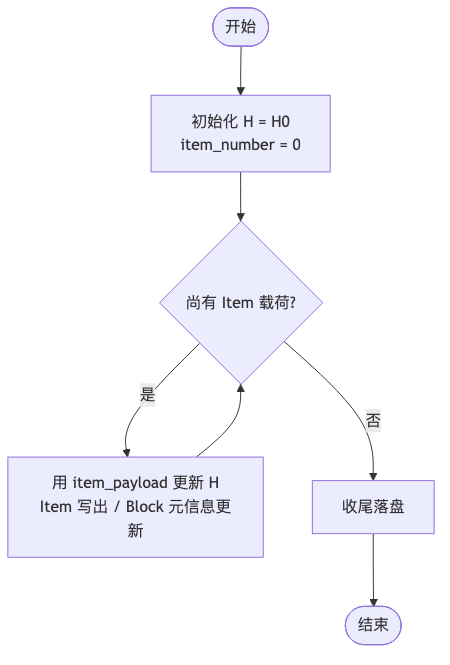
\includegraphics[width=0.85\textwidth]{diagrams/seal-main-flow.png}
  \caption{封装主循环（参考流程；Header.\ttf{tree_*} 由封装上下文提供，见图注及第~\ref{sec:seal-context} 节）}
  \label{fig:seal-main-flow}
\end{figure}

\textbf{实施步骤：}
以下按图~\ref{fig:seal-main-flow} 解读；各步以对应子节为准。
\begin{enumerate}
  \item \textbf{开始与初始化}（图：\texttt{开始}）：准备封装上下文（\ttf{magic_number}、\ttf{version_number} 等）；\ttf{block_number} $= 0$，\ttf{item_number} $= 0$；$H \leftarrow H_0$。无目录树时封装上下文 SHOULD 含 \ttf{tree_item_number} $=$ \texttt{0}。
  \item \textbf{主循环}（图：判断「尚有 Item 载荷」，取\textbf{是}）：集成层提供下一条 \ttf{item_payload}，调用第~\ref{sec:item-generation} 节（含 $H$ 更新与内容区写出），再调用第~\ref{sec:block-meta} 节；返回本步判断。
  \item \textbf{输入结束}（图：判断取\textbf{否}）：确认封装上下文中的 \ttf{tree_item_index}、\ttf{tree_item_number} 与已写 Item 布局一致后，按第~\ref{sec:seal-finalize} 节收尾（\ttf{data_hash} 写入 $H_n$，\ttf{tree_*} 自封装上下文写入 Header）。
\end{enumerate}

\subsection{封装一致性要求}\label{sec:seal-consistency}
\begin{itemize}
  \item 物理写入顺序 MUST 为：内容区 $\rightarrow$ Block Infos 区 $\rightarrow$ Header；
  \item \ttf{item_number} MUST 等于内容区实际 Item 条数；
  \item \ttf{block_number} MUST 等于 Block Infos 区条目数；
  \item 任意 Block Info 的 \ttf{end_file_pos} MUST 不超过 \ttf{content_size}，且相邻 Block 的偏移 SHOULD 首尾相接；
  \item 实现 SHOULD 在封装结束后校验计数与 Header.\ttf{data_hash} 按第~\ref{sec:rolling-hash} 节重算结果一致；
  \item 当 Header.\ttf{tree_item_number} $>$ \texttt{0} 时，\ttf{tree_item_index} 与 \ttf{tree_item_number} MUST 与内容区中目录树 Item 的实际范围一致，且目录树 \ttf{item_payload} 解析后 MUST 满足第~\ref{sec:directory-tree-chapter} 章（规划与校验见第~\ref{sec:multi-file-chapter} 章）。
\end{itemize}

\section{解封流程（参考）}\label{sec:unseal-chapter}

\subsection{与多文件、目录树的关系}\label{sec:unseal-byte-stream-scope}

本章规定从 \texttt{.sealed} 按 Item 顺序还原各条 \ttf{item_payload} 并由集成层得到 \ttf{payload}，与密封包内包含几个逻辑文件无关。
将 Item 序列按目录树还原为宿主侧目录结构，属于第~\ref{sec:multi-file-chapter} 章\textbf{整包解封}（目录明文见第~\ref{sec:directory-tree-chapter} 章）；本章仅规定 Item 级认证解密与 \ttf{data_hash} 校验，不重复整包还原步骤。
本章给出从 \texttt{.sealed} 文件按序还原业务载荷的\textbf{参考流程}。
\textbf{文件格式与可验证约束}以第~\ref{sec:format-chapter}、\ref{sec:crypto-chapter} 章为准；解封以 Item 为最小读取与认证单元，\ttf{item_payload} 须满足第~\ref{sec:item-payload-norms} 节且与封装侧同一集成语义。第~\ref{sec:format-chapter} 章「规范性解析流程」中的 MUST 条款在全量顺序解封时与本章一致，本章侧重步骤组合与图示。下文各节为信息性步骤说明，除非某条明确要求校验或布局。

\textbf{子流程（独立说明）：}
\begin{itemize}
  \item Header 获取与校验（第~\ref{sec:unseal-header-model} 节）；
  \item 内容区顺序读取（第~\ref{sec:unseal-item-parse} 节）；
  \item 单条 Item 认证解密（第~\ref{sec:unseal-item-crypto} 节）；
  \item Item 载荷输出与滚动摘要（第~\ref{sec:unseal-item-output} 节）；
  \item 解封流程总览（第~\ref{sec:unseal-total-algorithm} 节，含主循环图、完整性比对与组合调度）；
  \item 进度与可恢复状态（第~\ref{sec:unseal-recoverable} 节，建议性）。
\end{itemize}
上述步骤的\textbf{组合调度}见第~\ref{sec:unseal-total-algorithm} 节；全局一致性见第~\ref{sec:unseal-consistency} 节；失败语义见第~\ref{sec:unseal-errors} 节。

\subsection{Header 获取与校验}\label{sec:unseal-header-model}
从 \texttt{.sealed} 文件尾部取得 Header 记录，校验识别字段并计算三区长度（读取顺序见第~\ref{sec:read-model} 节）。

\textbf{输入：}
\begin{itemize}
  \item 已打开的 \texttt{.sealed} 文件及 \ttf{file_size}（见第~\ref{sec:region-length} 节）；
  \item \ttf{magic_number}、\ttf{version_number} 的约定取值（见第~\ref{sec:header-compat} 节）。
\end{itemize}

\textbf{输出：}
\begin{itemize}
  \item \ttf{block_number}、\ttf{item_number}、\ttf{data_hash}；
  \item \ttf{tree_item_index}、\ttf{tree_item_number}（自 Header 解析；Item 级主循环\textbf{不}依赖二者，整包解封见第~\ref{sec:multi-file-chapter} 章）；
  \item \ttf{content_size}、\ttf{block_infos_size}（由 \ttf{file_size} 与 \ttf{block_number} 按第~\ref{sec:region-length} 节算出）。
\end{itemize}

\textbf{相关格式：}
Header 记录布局见第~\ref{sec:header-region} 节；\ttf{data_hash} 字段语义见第~\ref{sec:rolling-hash} 节。

\textbf{实施步骤：}
\begin{enumerate}
  \item 读取文件末尾 80 字节，按第~\ref{sec:header-region} 节解析，得到各 Header 字段；
  \item 将解析得到的 \ttf{magic_number}、\ttf{version_number} 与\textbf{输入}中的约定取值比对；不符时 MUST 终止解封，错误码 SHOULD 为附录 C 中的 \ttf{E_MAGIC_MISMATCH} 或 \ttf{E_VERSION_UNSUPPORTED}；
  \item 令 \ttf{N} $=$ \ttf{block_number}，按第~\ref{sec:region-length} 节计算 \ttf{block_infos_size} 与 \ttf{content_size}；若 \ttf{content_size} 不大于 \texttt{0}，MUST 终止解封，错误码 SHOULD 为附录 C 中的 \ttf{E_FORMAT_TOO_SMALL}（或等价格式错误码）。
\end{enumerate}

\textbf{说明：}
全文件顺序解封\textbf{不必}事先读取 Block Infos 区；块级随机访问须先读 Block Infos 区（见第~\ref{sec:random-access-chapter} 章）。

\subsection{内容区顺序读取}\label{sec:unseal-item-parse}
本节说明全文件顺序解封时，如何从内容区切分出单条 Item 的 \ttf{item_size} 与 \ttf{cipher_payload}。

\textbf{输入：}
\begin{itemize}
  \item \ttf{content_size}、\ttf{item_number}（由第~\ref{sec:unseal-header-model} 节得到）。
\end{itemize}

\textbf{维护的状态：}
与第~\ref{sec:unseal-total-algorithm} 节主循环共享，本节负责在读每条 Item 后更新：
\begin{itemize}
  \item $p$：内容区读指针（相对内容区起点，单位：字节；初值 $p \leftarrow 0$ 见第~\ref{sec:unseal-total-algorithm} 节）；
  \item $n$：已处理 Item 计数（供主循环终止判断及完整性比对；初值 $n \leftarrow 0$ 见同上）。
\end{itemize}

\textbf{输出：}
\begin{itemize}
  \item 本条 Item 的 \ttf{item_size}（记为 $L$）与 \ttf{cipher_payload}。
\end{itemize}

\textbf{相关格式：}
内容区布局见第~\ref{sec:region-length}、\ref{sec:content-region} 节；Item 记录为 \texttt{[item\_size (8B)][cipher\_payload (L B)]}（见第~\ref{sec:item-record}、\ref{sec:cipher-payload-layout} 节）。\textbf{条数不由扫描推断}，以 \ttf{item_number} 为终止条件。本节\textbf{每次调用}读取\textbf{一条} Item。

\textbf{实施步骤：}
\begin{enumerate}
  \item 若 \ttf{content_size} $-$ $p < 8$，MUST 终止本条 Item 读取，错误码 SHOULD 为附录 C 中的 \ttf{E_ITEM_TRUNCATED}；
  \item 自偏移 $p$ 起读取 8 字节，解码为 $L$；若 $L$ 非法（如为 \texttt{0} 或超出实现上限），MUST 终止解封，错误码 SHOULD 为附录 C 中的 \ttf{E_ITEM_SIZE_INVALID}；
  \item 若 \ttf{content_size} $-$ $p < 8 + L$，MUST 终止本条 Item 读取，错误码 SHOULD 为附录 C 中的 \ttf{E_ITEM_TRUNCATED}；
  \item 自偏移 $p + 8$ 起读取 $L$ 字节，得到 \ttf{cipher_payload}；若其布局不满足第~\ref{sec:cipher-payload-layout} 节，MUST 终止解封，错误码 SHOULD 为附录 C 中的 \ttf{E_ITEM_SIZE_INVALID}；
  \item 更新 $p \leftarrow p + 8 + L$、$n \leftarrow n + 1$；当 $n = \ttf{item_number}$ 时，若 $p \ne \ttf{content_size}$，MUST 终止解封（格式错误，如 \ttf{E_ITEM_TRUNCATED} 或实现自定义码）。
\end{enumerate}

\textbf{说明：}
解密与 \ttf{payload} 输出不在本节展开；见第~\ref{sec:unseal-item-crypto}、\ref{sec:unseal-item-output} 节及第~\ref{sec:unseal-total-algorithm} 节。

\subsection{单条 Item 认证解密}\label{sec:unseal-item-crypto}
将一条 Item 的密文载荷还原为 \ttf{item_payload}。

\textbf{输入：}
\begin{itemize}
  \item \ttf{cipher_payload}（由第~\ref{sec:unseal-item-parse} 节读出）；
  \item 接收方长期私钥（应用层提供，见第~\ref{sec:curve-keys} 节）。
\end{itemize}

\textbf{输出：}
\begin{itemize}
  \item \ttf{item_payload}（认证成功后）。
\end{itemize}

\textbf{实施步骤：}
\begin{enumerate}
  \item 对 \ttf{cipher_payload} 与接收方长期私钥调用第~\ref{sec:decrypt-crypto} 节内容解密还原模块；
  \item 若认证失败（第~\ref{sec:auth-failure} 节），MUST 终止解封，MUST NOT 输出 \ttf{item_payload}，错误码 SHOULD 为附录 C 中的 \ttf{E_AEAD_AUTH_FAILED}；
  \item 认证成功时，得到 \ttf{item_payload}。
\end{enumerate}

\textbf{说明：}
算法细节见第~\ref{sec:decrypt-crypto} 节；本章不重复模块内部步骤。

\subsection{Item 载荷输出与滚动摘要}\label{sec:unseal-item-output}\label{sec:unseal-rolling-hash}\label{sec:unseal-batch-output}
将一条 Item 解密得到的 \ttf{item_payload} 用于更新滚动摘要 $H$，并由集成层输出对应的 \ttf{payload}。

\textbf{输入（每次调用）：}
\ttf{item_payload}（由第~\ref{sec:unseal-item-crypto} 节得到）。

\textbf{维护的状态：}
$H$：滚动摘要状态（$H_0$ 见第~\ref{sec:rolling-hash} 节；初值与调度见第~\ref{sec:unseal-total-algorithm} 节）。

\textbf{输出（每次调用）：}
本条 Item 对应的 \ttf{payload}（由集成层从 \ttf{item_payload} 还原）。

\textbf{相关格式：}
\ttf{item_payload} 须满足第~\ref{sec:item-payload-norms} 节；$H$ 递推见第~\ref{sec:rolling-hash}、\ref{sec:rolling-hash-final} 节。

\textbf{实施步骤：}
\begin{enumerate}
  \item 在输出 \ttf{payload} 之前，用本条 \ttf{item_payload} 完整字节串按第~\ref{sec:rolling-hash} 节更新 $H$；
  \item 由集成层将 \ttf{item_payload} 还原为 \ttf{payload} 并输出；语义须与封装侧一致；失败时 MUST 终止解封（格式错误）。
\end{enumerate}

\textbf{说明：}
$H$ 的累计顺序 MUST 与封装侧 Item 顺序一致。完整性比对见第~\ref{sec:unseal-total-algorithm} 节。

\subsection{解封流程总览}\label{sec:unseal-total-algorithm}\label{sec:unseal-main-flow}
本节定义解封侧\textbf{如何组合}前述子流程。各子节仅描述单步职责；本节给出调度变量、主循环参考图及\textbf{按图解读}的实施步骤（含完整性比对）。

\textbf{变量与状态（仅在本节及图中使用）：}
\begin{itemize}
  \item 内容区读指针 $p$、已处理 Item 计数 $n$（由第~\ref{sec:unseal-item-parse} 节维护）；
  \item 滚动摘要状态 $H$（由第~\ref{sec:unseal-item-output} 节维护；$H_0$ 见第~\ref{sec:rolling-hash} 节）；
  \item \ttf{item_number}、\ttf{content_size}、\ttf{data_hash}（由第~\ref{sec:unseal-header-model} 节得到）。
\end{itemize}

\textbf{主循环图与子节对应：}
图~\ref{fig:unseal-main-flow} 为全量顺序解封的一种参考主流程；图源 \texttt{doc/diagrams/unseal-main-flow.mmd}。
图中流程名词与独立子节的对应关系如下（图中\textbf{不}标注章节号；\ttf{data_hash} 等字段语义以正文为准）：
\begin{itemize}
  \item 「读 Header 并校验」「计算 \ttf{content_size}」：见第~\ref{sec:unseal-header-model} 节；图中「初始化 $H = H_0$，$n = 0$」另需 $p \leftarrow 0$（$H_0$ 见第~\ref{sec:rolling-hash} 节）；
  \item 「读 \ttf{item_size} 与 \ttf{cipher_payload}」：见第~\ref{sec:unseal-item-parse} 节（含 $n$ 递增，图中无单独「$n$ 加 1」节点）；
  \item 「认证解密得 Item 载荷」：见第~\ref{sec:unseal-item-crypto} 节；
  \item 「输出 \ttf{payload} 并用 Item 载荷更新 $H$」：见第~\ref{sec:unseal-item-output} 节（须在输出 \ttf{payload} 之前更新 $H$）；
  \item 「$H$ 等于 \ttf{data_hash}」：见下文实施步骤第 3 项（完整性比对）。
\end{itemize}

\begin{figure}[htbp]
  \centering
  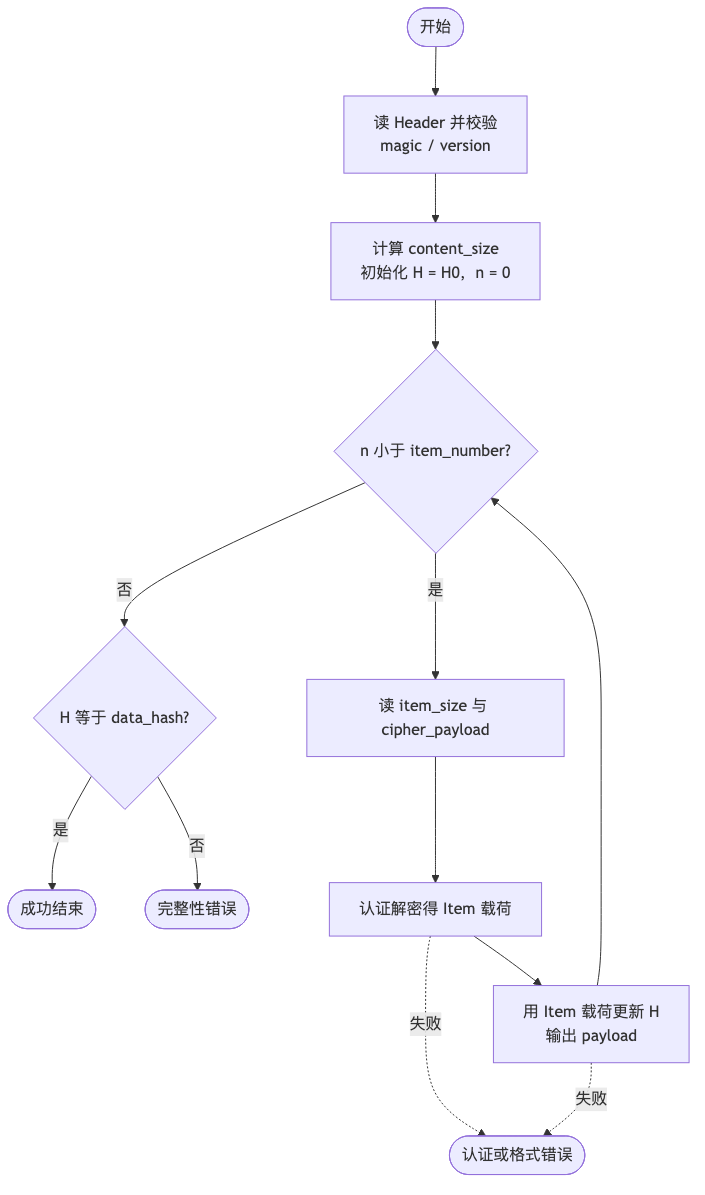
\includegraphics[width=0.85\textwidth]{diagrams/unseal-main-flow.png}
  \caption{解封主循环（参考流程，全量顺序解封）}
  \label{fig:unseal-main-flow}
\end{figure}

\textbf{实施步骤：}
以下按图~\ref{fig:unseal-main-flow} 自上而下解读；各步具体操作以对应子节为准。
\begin{enumerate}
  \item \textbf{开始与 Header}（图：\texttt{开始} $\rightarrow$ 「读 Header 并校验」$\rightarrow$ 「计算 \ttf{content_size} / 初始化」）：按第~\ref{sec:unseal-header-model} 节取得并校验 Header；$H \leftarrow H_0$，$p \leftarrow 0$，$n \leftarrow 0$。
  \item \textbf{主循环}（图：判断 $n$ 小于 \ttf{item_number}，取\textbf{是}）：以当前 $p$、$n$ 调用第~\ref{sec:unseal-item-parse} 节得 \ttf{cipher_payload} 及更新后的 $p$、$n$；调用第~\ref{sec:unseal-item-crypto} 节得 \ttf{item_payload}；以当前 $H$ 调用第~\ref{sec:unseal-item-output} 节输出 \ttf{payload} 并更新 $H$；然后返回本步判断。认证或格式失败时 MUST 终止（图虚线至错误结束）。
  \item \textbf{完整性比对}\label{sec:integrity-check}（图：$n$ 判断取\textbf{否} $\rightarrow$ 「$H$ 等于 \ttf{data_hash}」）：将 $H$ 与 \ttf{data_hash} 逐字节比较；相等则成功结束，不等则 MUST 终止解封，错误码 SHOULD 为附录 C 中的 \ttf{E_INTEGRITY_MISMATCH}，并视已输出的 \ttf{payload} 为不可信；流式输出时 SHOULD 停止下游消费并上报错误。
\end{enumerate}

\subsection{错误处理}\label{sec:unseal-errors}
下列情况 MUST 立即失败，且\textbf{不得}继续输出后续 \ttf{payload}（已输出部分视实现策略可标记为不可信）：
\begin{itemize}
  \item \ttf{magic_number} 或 \ttf{version_number} 校验失败（第~\ref{sec:header-compat} 节）；
  \item \ttf{content_size} 非法，或第~\ref{sec:unseal-item-parse} 节读取 Item 时字节不足或布局非法；
  \item 第~\ref{sec:decrypt-crypto} 节内容解密还原模块认证失败（第~\ref{sec:auth-failure} 节）；
  \item 第~\ref{sec:unseal-item-output} 节 Item 载荷解码或 \ttf{payload} 还原失败；
  \item 第~\ref{sec:unseal-total-algorithm} 节完整性比对中 $H$ 与 \ttf{data_hash} 不一致。
\end{itemize}

\subsection{解封一致性要求}\label{sec:unseal-consistency}
\begin{itemize}
  \item 输出的各段 \ttf{payload} 全局顺序 MUST 与封装侧提交的载荷顺序一致；
  \item 每条 \ttf{payload} MUST 来自经第~\ref{sec:decrypt-crypto} 节认证成功的 \ttf{item_payload}；
  \item 处理完全部 Item 后，$H$ MUST 与 \ttf{data_hash} 一致；
  \item 全文件顺序解封时，实际读取的 Item 条数 MUST 等于 \ttf{item_number}；
  \item 失败时 MUST 符合第~\ref{sec:unseal-errors} 节，不得静默跳过损坏 Item 继续输出。
\end{itemize}

\subsection{进度与可恢复状态（建议）}\label{sec:unseal-recoverable}
支持断点续传或分块交付的实现，在恢复语义下 SHOULD 持久化并可恢复下列状态（名称可因实现而异）：
\begin{itemize}
  \item 已完成处理的 Item 数（对应 $n$）；
  \item 内容区读指针 $p$（含已读 \texttt{item\_size} 前缀与 \ttf{cipher_payload}）；
  \item 滚动摘要状态 $H$（规则 MUST 与第~\ref{sec:rolling-hash} 节一致）；
  \item 已提交给下游的 \ttf{payload} 字节进度；
  \item 已解密但尚未全部交付下游的缓冲（若存在）。
\end{itemize}

\textbf{说明：}
写入端与读取端 MUST 在同一恢复语义下同步推进密文读取偏移与明文提交偏移，避免重复输出或跳写；调度见图~\ref{fig:unseal-main-flow}。

% 第 9 章：目录树明文格式（框架）
% 规定目录（树）逻辑文件的明文布局、解析与校验；生成与整包还原见第 10 章。

\section{目录树明文格式}\label{sec:directory-tree-chapter}

自本版起，通过\textbf{目录树文件}在单条 \texttt{.aeff} 内索引多个逻辑文件与子目录：封装时将宿主侧目录树（各文件的\textbf{相对路径}与层级）写入目录明文，解封后在集成层指定的输出根路径下按相同相对路径还原，以保留与密封前一致的目录结构（第~\ref{sec:multi-file-chapter} 章给出封装与整包解封流程）。

\subsection{定位}\label{sec:directory-tree-scope}

\begin{itemize}
  \item \textbf{目录（树）文件}：密封包内的一份逻辑文件，其明文为下文规定的目录索引字节布局；在 Content Region 中与其它逻辑文件一样，经 Item 加密存储（第~\ref{sec:content-region} 节）。\textbf{目录项}（\ttf{dir_item}）与\textbf{文件项}（\ttf{file_entry}）等记录类型见第~\ref{sec:tree-string-section} 节起各小节。
  \item 本章规定目录明文的\textbf{二进制布局、解析与校验}；封装侧如何\textbf{生成}该明文、Header 目录树 Item 定位字段如何取值及解封侧如何\textbf{消费}解析结果，见附录~\ref{sec:multi-file-chapter}。
  \item 本章\textbf{不}重复附录~\ref{sec:unseal-chapter} 的 Item 认证解密步骤；解封侧须先按附录~\ref{sec:multi-file-tree-payload-concat} 得到目录明文字节串，再调用本章解析。
\end{itemize}

\subsection{无目录树情形}\label{sec:directory-tree-no-tree}

当 Header.\ttf{tree_item_number} $=$ \texttt{0} 时，本标准\textbf{不}要求存在符合本章布局的目录明文；多文件整包还原流程不适用，解封侧 MAY 仅按第~\ref{sec:unseal-chapter} 章输出 Item 序列。互操作细则见第~\ref{sec:multi-file-no-tree} 节。

\subsection{规范约定}\label{sec:directory-tree-conventions}

\begin{itemize}
  \item 除特别说明外，整数类型均为无符号，多字节整数均为小端序（LE）；
  \item 本章所称\textbf{目录明文}，指解密目录树 Item 后得到的连续字节串；下文偏移均以目录明文\textbf{首字节为 0} 计量；
  \item 字段名使用下划线命名，与实现互操作对齐；
  \item 目录树明文格式版本由树头.\ttf{version} 表示，与 \texttt{.aeff} 文件 Header.\ttf{version_number} \textbf{相互独立}；当前版本约定值见第~\ref{sec:tree-header} 节（暂定）。
\end{itemize}

\subsection{整体布局}\label{sec:tree-file-layout}

目录明文是解密目录树 Item 后得到的一段连续字节串，用于描述密封包内目录层级、各逻辑文件及其与 Content Region 中 Item 的对应关系。自目录明文首字节起，按从前到后顺序布局如下：
\begin{center}
  \texttt{[树头][目录节][文件节][符号节]}
\end{center}
\begin{itemize}
  \item \textbf{树头}：固定 40 字节，含魔数、版本及后三节起始偏移，详见第~\ref{sec:tree-header} 节；
  \item \textbf{目录节}：紧密存放全部目录项（\ttf{dir_item}），见第~\ref{sec:tree-dir-section} 节；
  \item \textbf{文件节}：紧密存放全部文件项（\ttf{file_entry}），见第~\ref{sec:tree-file-section} 节；
  \item \textbf{符号节}：紧密存放 NUL 结尾的 UTF-8 名称串，见第~\ref{sec:tree-string-section} 节。
\end{itemize}
各节边界由树头定位字段给出；下文按「树头 $\rightarrow$ 符号节 $\rightarrow$ 文件节 $\rightarrow$ 目录节」叙述。
各节边界由树头中的定位字段给出。

\subsection{树头}\label{sec:tree-header}

树头位于目录明文偏移 \texttt{0} 处，长度固定为 40 字节。字段布局如下：

\begin{longtable}{>{\raggedright\arraybackslash}p{3.4cm} >{\raggedright\arraybackslash}p{1.2cm} >{\raggedright\arraybackslash}p{1.2cm} >{\raggedright\arraybackslash}p{6.6cm}}
  \toprule
  字段名 & 偏移 & 长度 & 说明 \\
  \midrule
  \endhead
  \ttf{magic_number} & 0 & 8 & 目录明文魔数（\ttf{UINT64(LE)}，见下文参考约定） \\
  \ttf{version} & 8 & 8 & 目录明文格式版本（\ttf{UINT64(LE)}，见下文参考约定） \\
  \ttf{dir_offset} & 16 & 8 & 目录节在目录明文内的起始偏移（\ttf{UINT64(LE)}） \\
  \ttf{file_offset} & 24 & 8 & 文件节在目录明文内的起始偏移（\ttf{UINT64(LE)}） \\
  \ttf{str_offset} & 32 & 8 & 符号节在目录明文内的起始偏移（\ttf{UINT64(LE)}） \\
  \bottomrule
\end{longtable}

\textbf{补充说明：}
\begin{itemize}
  \item \ttf{magic_number}、\ttf{version}：读取器 MUST 在进入后续解析前完成校验（失败语义见第~\ref{sec:directory-tree-parse} 节）；
  \item \ttf{dir_offset}、\ttf{file_offset}、\ttf{str_offset}：实现 MUST 校验 $0 \le \mathit{dir\_offset} \le \mathit{file\_offset} \le \mathit{str\_offset} \le \mathit{plaintext\_len}$（细则见第~\ref{sec:directory-tree-parse} 节校验步骤 1）。
\end{itemize}

\noindent\textbf{参考约定参数（当前版本，暂定）：}\label{sec:tree-header-params}
为保证目录明文互操作，当前约定 \ttf{version = 2}（\ttf{UINT64(LE)}，暂定；\ttf{file_entry} 为 72 字节且含 \ttf{restore_flag}）。
\ttf{magic_number}（\ttf{UINT64(LE)}，8 字节，暂定）为：字符串形式 ASCII \texttt{YEEZTRID}（恰好 8 字节，\textbf{无}结尾 \texttt{0x00}）；十六进制（自目录明文偏移 \texttt{0} 起连续 8 字节）：\texttt{5945455a54495245}。
树头.\ttf{version} 仅描述目录明文布局演进，与 \texttt{.aeff} Header.\ttf{version_number} \textbf{无}对应关系，二者 MAY 独立递增；读取器 MUST 在解析目录节前校验 \ttf{magic_number} 与 \ttf{version}；若后续调整树头布局或上述常量，树头.\ttf{version} MUST 递增并提供兼容说明，\textbf{不必}与 aeff 文件版本同步。

\subsection{符号节}\label{sec:tree-string-section}

符号节为目录明文中自 \ttf{str_offset} 起至目录明文末尾的字节区间，供后文 \ttf{dir_item}、\ttf{file_entry} 的 \ttf{name} 字段引用。每段为\textbf{单层}目录名或文件名（\textbf{不}含 \texttt{/}、\texttt{\textbackslash}），用于第~\ref{sec:multi-file-chapter} 章整包还原时在宿主侧拼接相对路径。

\textbf{编码策略：} 各名称串按 UTF-8 编码（\textbf{无} BOM），在符号节内\textbf{首尾相接、紧密排列}；每段以单个 \texttt{0x00}（NUL）结尾，段与段之间\textbf{无}额外长度前缀或填充字节。布局示意：
\begin{center}
  \small
  \texttt{[UTF-8 名称字节…][0x00][UTF-8 名称字节…][0x00]…}
\end{center}

\begin{itemize}
  \item \ttf{name}（\ttf{UINT32(LE)}）为\textbf{符号节内字节偏移}：名称起点 $=$ \ttf{str_offset} $+$ \ttf{name}；解析器 MUST 自该起点按字节读至首个 \texttt{0x00} 为止（\textbf{无}独立长度字段）；
  \item 空名称（根目录项）：\ttf{name} 所指向处首字节 MUST 为 \texttt{0x00}（即仅含终止符的一段）；
  \item 名称正文 MUST 为合法 UTF-8，且 MUST NOT 在终止符之前出现 \texttt{0x00}；
  \item 多条记录 MAY 共用同一 \ttf{name} 偏移（相同名称只存一份）；
  \item 封装侧 MAY 按任意顺序写入各段；解析器 MUST 仅通过 \ttf{name} 偏移定位字符串，不得假设全局字典序；
  \item 符号节内所有被引用的 \ttf{name} 偏移 MUST 落在符号节区间内，且 MUST 能在该区间内扫描到终止符；否则 MUST 判为格式错误；
  \item 自目录树还原宿主侧相对路径及写回目录结构的规则见第~\ref{sec:multi-file-chapter} 章，本章不定义路径拼接算法。
\end{itemize}

\subsection{文件节与文件项}\label{sec:tree-file-section}
\label{sec:tree-file-entry}

文件节为目录明文中 $[$\ttf{file_offset},\ \ttf{str_offset}$)$ 字节区间，自 \ttf{file_offset} 起由 $M$ 条\textbf{文件项}（\ttf{file_entry}）紧密排列；每条固定 72 字节，描述一个逻辑文件在 Content Region 中的位置及元数据。字段布局如下：

\begin{longtable}{>{\raggedright\arraybackslash}p{3.4cm} >{\raggedright\arraybackslash}p{1.2cm} >{\raggedright\arraybackslash}p{1.2cm} >{\raggedright\arraybackslash}p{6.6cm}}
  \toprule
  字段名 & 偏移 & 长度 & 说明 \\
  \midrule
  \endhead
  \ttf{name} & 0 & 4 & 本逻辑文件文件名在符号节内的偏移（\ttf{UINT32(LE)}） \\
  \ttf{mtime} & 4 & 8 & 本逻辑文件末次修改时间：\ttf{UINT64(LE)}，自 Unix 纪元起的整秒数（UTC） \\
  \ttf{ctime} & 12 & 8 & 本逻辑文件创建时间：\ttf{UINT64(LE)}，自 Unix 纪元起的整秒数（UTC） \\
  \ttf{hash} & 20 & 32 & 逻辑文件明文摘要（\ttf{BYTESTRING[32]}）；算法由集成层定义，本标准\textbf{不}规定 \\
  \ttf{item_index} & 52 & 8 & 该逻辑文件首条 Item 在 Content Region 中的全局下标（\ttf{UINT64(LE)}，含） \\
  \ttf{item_number} & 60 & 8 & 该逻辑文件占用的连续 Item 条数（\ttf{UINT64(LE)}） \\
  \ttf{restore_flag} & 68 & 1 & 整包解封时是否写回宿主目录树（\ttf{UINT8(LE)}，见下文） \\
  \ttf{reserved} & 69 & 3 & 保留，当前版本 MUST 为 \texttt{0x00} \\
  \bottomrule
\end{longtable}

\textbf{\ttf{restore_flag} 取值：}
\begin{center}
  \small
  \begin{tabular}{cl}
    \toprule
    值 & 含义 \\
    \midrule
    \texttt{0} & 不写回宿主目录（辅助/索引/说明等；仍占用 Item，参与第 7 章解密与滚动摘要） \\
    \texttt{1} & 写回宿主目录（密封包中应出现在最终目录树中的逻辑文件） \\
    \bottomrule
  \end{tabular}
\end{center}
其它取值保留；解析器对当前目录明文 \ttf{version} MUST 判为格式错误。

\textbf{补充说明：}符号链接占一条 \ttf{file_entry}（字段同上），链接目标在 Item 载荷中，见第~\ref{sec:multi-file-symlink} 节。

\subsection{目录节与目录项}\label{sec:tree-dir-section}
\label{sec:tree-dir-item}

\textbf{术语：}
\begin{itemize}
  \item \textbf{目录}：目录树中的结点，可包含子目录子结点及逻辑文件子结点；层级关系由 \ttf{dir_item} 的 \ttf{children} 表达；
  \item \textbf{目录项}（\ttf{dir_item}）：目录节内描述一个目录的二进制记录（字段见下文），与目录一一对应；
  \item \textbf{根目录}：目录树入口，对应目录节中首条 \ttf{dir_item}（\ttf{name} 须为空，见下文补充说明）；
  \item \textbf{目录节}：目录明文中 $[$\ttf{dir_offset},\ \ttf{file_offset}$)$ 字节区间，紧密存放全部 \ttf{dir_item}。
\end{itemize}

\textbf{目录节与目录项的关系：}
目录节字节区间 $[$\ttf{dir_offset},\ \ttf{file_offset}$)$ 内，全部 \ttf{dir_item} 自 \ttf{dir_offset} 起按条紧密排列（首尾相接、无空隙），规则与第~\ref{sec:content-region} 节 Item 序列相同：
\begin{itemize}
  \item 每条 \ttf{dir_item} 对应一个目录；单条长度为 $24 + 8 \times N$ 字节，$N =$ \ttf{child_number}（见下表）；
  \item \textbf{第一条} MUST 为\textbf{根目录项}，起始偏移 MUST 等于 \ttf{dir_offset}；
  \item 其余 \ttf{dir_item} 紧接在前一条之后顺序写出；除「根目录项必须为首条」外，本标准\textbf{不}规定各目录项的先后顺序（封装侧 MAY 按生成算法任意排列）；
  \item 目录节内字节 MUST 被各 \ttf{dir_item} 恰好占满：最后一条 \ttf{dir_item} 的结束偏移 MUST 等于 \ttf{file_offset}，MUST NOT 存在尾部未使用字节。
\end{itemize}

解析器 MAY 自 \ttf{dir_offset} 顺序扫描并切分全部 \ttf{dir_item}，同时 MUST 自根目录项起按 \ttf{child} 递归遍历目录树；两种方式得到的目录项边界 MUST 一致。封装侧生成算法见第~\ref{sec:multi-file-chapter} 章。

\subsubsection{目录项（\texttt{dir\_item}）}

每条 \ttf{dir_item} 自其起始偏移起，按字节从前到后布局如下（$N =$ \ttf{child_number}，本条长度 $24 + 8N$ 字节）：
\begin{center}
  \texttt{[name (4B)][mtime (8B)][ctime (8B)][child\_number (4B)][child (8B)]$\times N$}
\end{center}
字段布局如下：
\begin{longtable}{>{\raggedright\arraybackslash}p{3.4cm} >{\raggedright\arraybackslash}p{1.2cm} >{\raggedright\arraybackslash}p{1.2cm} >{\raggedright\arraybackslash}p{6.6cm}}
  \toprule
  字段名 & 偏移 & 长度 & 说明 \\
  \midrule
  \endhead
  \ttf{name} & 0 & 4 & 本目录名称在符号节内的偏移（\ttf{UINT32(LE)}） \\
  \ttf{mtime} & 4 & 8 & 本目录末次修改时间（\ttf{UINT64(LE)}，Unix 纪元起整秒，UTC） \\
  \ttf{ctime} & 12 & 8 & 本目录创建时间（\ttf{UINT64(LE)}，Unix 秒，UTC） \\
  \ttf{child_number} & 20 & 4 & 子节点个数（\ttf{UINT32(LE)}） \\
  \ttf{children} & 24 & $8 \times N$ & 连续 $N =$ \ttf{child_number} 个\textbf{子节点}（\ttf{child}，各 8 字节），见第~\ref{sec:tree-child} 节 \\
  \bottomrule
\end{longtable}

\textbf{补充说明：}\textbf{根目录项}（首条 \ttf{dir_item}）的 \ttf{name} MUST 为\textbf{空}（符号节中仅 \texttt{0x00}）；\textbf{不得}用 \texttt{/}、\texttt{.}、\texttt{..} 代替。

\subsubsection{子节点（\texttt{child}）}\label{sec:tree-child}

每个 \ttf{child} 占 8 字节，编码为单个 \ttf{UINT64(LE)}，自低字节起按位打包如下（图中 \texttt{b} 表示\textbf{比特}，\textbf{非}字节 \texttt{B}）：
\begin{center}
  \texttt{[type (4b)][offset (60b)]}
\end{center}
按位含义：
\begin{itemize}
  \item 低 4 位 \ttf{type}：子结点对应的\textbf{宿主文件类型}；编码规则与取值表见附录~\ref{app:child-type-table}；
  \item 高 60 位 \ttf{offset}：目录明文内的绝对字节偏移（自目录明文首字节为 \texttt{0} 起算），为被引用记录的\textbf{首字节}位置。
\end{itemize}

\textbf{补充说明：}
\begin{itemize}
  \item \ttf{type} $=$ \texttt{4}（\texttt{S\_IFDIR}）时，\ttf{offset} MUST $\in [$\ttf{dir_offset},\ \ttf{file_offset}$)$ 且为某条 \ttf{dir_item} 边界；
  \item \ttf{type} $=$ \texttt{8}（\texttt{S\_IFREG}）或 \texttt{10}（\texttt{S\_IFLNK}）时，\ttf{offset} MUST $\in [$\ttf{file_offset},\ \ttf{str_offset}$)$ 且 $(\mathtt{offset}-\mathtt{file\_offset}) \bmod 72 = 0$；
  \item 其它 \ttf{type} 及越界 \ttf{offset} MUST 判为格式错误（禁止类型见附录~\ref{app:child-type-table}）。
\end{itemize}

\subsection{目录树明文解析与校验}\label{sec:directory-tree-parse}

本节规定对目录明文字节串的\textbf{规范性解析}（封装侧生成后自检、解封侧整包还原前校验均可调用）。调用方 MUST 传入 \texttt{content\_item\_number}（Content Region 中 Item 总条数；解封时通常取 Header.\ttf{item_number}），用于校验文件记录下标不越界。

\begin{algorithm}[htbp]
\caption{目录树遍历框架（供校验与还原共同引用）}
\label{alg:tree-visit}
\begin{algorithmic}[1]
\Require 目录明文字节串；树头与各节偏移已完成基本校验
\State $\mathit{visited} \gets \emptyset$；$\mathit{path\_stack} \gets []$
\State $\mathit{file\_leaf\_count} \gets 0$；$\mathit{seen\_file\_offsets} \gets \emptyset$ \Comment{校验：判重复引用}
\Procedure{Visit}{$p$}
  \If{$p \notin [\mathit{dir\_offset},\ \mathit{file\_offset})$ \textbf{ or } $p \in \mathit{visited}$}
    \State \textbf{报错并终止}
  \EndIf
  \State $\mathit{visited} \gets \mathit{visited} \cup \{p\}$
  \State 读取当前 \ttf{dir_item}；$\mathit{len} \gets 24 + 8 \times \mathit{child\_number}$
  \If{$p + \mathit{len} > \mathit{file\_offset}$}
    \State \textbf{报错并终止}
  \EndIf
  \State \textbf{目录结点动作}（校验：验证 \ttf{name} 偏移合法；还原：按 $\mathit{path\_stack}$ 建目录并设置时间）
  \For{$k \gets 0$ \textbf{to} $\mathit{child\_number}-1$}
    \State 读取第 $k$ 个 \ttf{child}，得 $\mathit{type}$、$\mathit{offset}$
    \If{$\mathit{type} \in \{1,2,6,12\}$ \textbf{ or } $\mathit{type}$ 为其它保留值}
      \State \textbf{报错并终止} \Comment{禁止 \texttt{S\_IFIFO}/\texttt{S\_IFCHR}/\texttt{S\_IFBLK}/\texttt{S\_IFSOCK} 等}
    \ElsIf{$\mathit{type} = 4$}
      \If{$\mathit{offset} \notin [\mathit{dir\_offset},\ \mathit{file\_offset})$}
        \State \textbf{报错并终止}
      \EndIf
      \State 子目录名压入 $\mathit{path\_stack}$；\Call{Visit}{$\mathit{offset}$}；弹出 $\mathit{path\_stack}$
    \ElsIf{$\mathit{type} \in \{8, 10\}$}
      \If{$(\mathit{offset}-\mathit{file\_offset}) \bmod 72 \neq 0$ \textbf{ or } $\mathit{offset} \notin [\mathit{file\_offset},\ \mathit{str\_offset})$}
        \State \textbf{报错并终止}
      \EndIf
      \If{$\mathit{offset} \in \mathit{seen\_file\_offsets}$}
        \State \textbf{报错并终止} \Comment{同一 \ttf{file_entry} 不得被多个 \ttf{child} 引用}
      \EndIf
      \State $\mathit{seen\_file\_offsets} \gets \mathit{seen\_file\_offsets} \cup \{\mathit{offset}\}$；$\mathit{file\_leaf\_count} \gets \mathit{file\_leaf\_count} + 1$
      \State \textbf{叶结点动作} \Comment{校验：读 \ttf{file_entry}，校验 \ttf{restore_flag} 与 Item 下标；还原：见第 10 章}
    \Else
      \State \textbf{报错并终止}
    \EndIf
  \EndFor
\EndProcedure
\State \Call{Visit}{$\mathit{dir\_offset}$}
\end{algorithmic}
\end{algorithm}

\noindent\textbf{说明：}还原侧可忽略 $\mathit{file\_leaf\_count}$、$\mathit{seen\_file\_offsets}$。校验侧 $\mathit{seen\_file\_offsets}$ 仅用于发现「多个 \ttf{child} 指向同一 \ttf{file_entry}」；遍历结束后在禁止重复引用的前提下，$\mathit{file\_leaf\_count} = M$ 即等价于文件节 $M$ 条记录均被引用且无孤儿（因合法 \ttf{offset} 在文件节内 72 字节对齐且至多 $M$ 个槽位）。

\subsubsection*{校验步骤}

记目录明文总长度为 $\mathit{plaintext\_len}$，文件节条数
\[
  M = \frac{\mathit{str\_offset} - \mathit{file\_offset}}{72}
\]
须为整数；否则 MUST 报错并终止。

\begin{enumerate}
  \item 读取并校验树头（第~\ref{sec:tree-header} 节）：\ttf{magic_number}、\ttf{version}；且 $0 \le \mathit{dir\_offset} \le \mathit{file\_offset} \le \mathit{str\_offset} \le \mathit{plaintext\_len}$；
  \item 调用算法~\ref{alg:tree-visit}（自 \ttf{dir_offset} 起）完成目录树遍历；$\mathit{file\_leaf\_count}$ 须等于 $M$（算法内已对重复 \ttf{offset} 报错，故无需再单独比较集合大小）；
  \item 线性扫描符号节：凡在遍历中被引用的 \ttf{name} 偏移，均须落在 $[\mathit{str\_offset},\ \mathit{plaintext\_len})$ 内且能读到 NUL 终止符；
  \item 上述步骤全部通过则校验成功；否则 MUST 终止后续整包还原（错误码见附录~\ref{sec:directory-tree-errors}）。
\end{enumerate}

% 附录 G：多文件封装与解封（参考）
% 在 Item 管道（附录 H）之上编排多逻辑文件与目录树；目录明文格式见第 7 章。

\section{附录 G：多文件封装与解封（参考）}\label{sec:multi-file-chapter}

\subsection{定位与依赖}\label{sec:multi-file-scope}

本章描述多文件场景下的\textbf{外层编排}，以附录~\ref{app:seal-unseal-reference} Item 管道为执行层，不修改其内部步骤。

\begin{itemize}
  \item 附录~\ref{app:seal-unseal-reference} 只处理\textbf{按序 Item 载荷}，不感知宿主目录结构。
  \item 本章在附录~\ref{app:seal-unseal-reference}之上完成三件事：
        \begin{enumerate}
          \item 扫描宿主目录，生成\textbf{目录树文件}（明文格式见第~\ref{sec:directory-tree-chapter} 章）；
          \item 为目录树文件和各数据文件分配全局 Item 下标；
          \item 按分配结果组装写出队列，调用附录~\ref{app:seal-unseal-reference}写入 \texttt{.aeff}，收尾时写入 Header。
        \end{enumerate}
  \item 目录树\textbf{二进制布局}见第~\ref{sec:directory-tree-chapter} 章；符号链接 Item 编码见第~\ref{sec:multi-file-symlink} 节；解封后的整包还原见第~\ref{sec:multi-file-unseal-restore} 节。
  \item 除明确援引格式或校验条款外，本章步骤为\textbf{参考性}说明；Item 切分粒度、路径拼接、摘要算法等由集成层声明，\textbf{不}写入 \texttt{.aeff} 物理布局。
\end{itemize}

\textbf{子流程（独立说明）：}
\begin{itemize}
  \item 无目录树与单流包（第~\ref{sec:multi-file-no-tree} 节）；
  \item 目录树文件生成（第~\ref{sec:multi-file-tree-generate} 节）；
  \item 全局 Item 分配与 Header 目录树定位（第~\ref{sec:multi-file-item-alloc} 节）；
  \item 多文件封装总流程（第~\ref{sec:multi-file-seal-flow} 节）；
  \item 整包解封与多文件还原（第~\ref{sec:multi-file-unseal-restore} 节）；
  \item 逻辑文件写回标记（第~\ref{sec:multi-file-restore-flag} 节）；
  \item 符号链接 Item 载荷与写回（第~\ref{sec:multi-file-symlink} 节）；
  \item 一致性与错误处理（第~\ref{sec:multi-file-consistency} 节）。
\end{itemize}

\subsection{无目录树与单流包}\label{sec:multi-file-no-tree}

当密封包不含目录索引（Header.\ttf{tree_item_number} $=$ \texttt{0}）时：

\begin{itemize}
  \item 封装侧 MAY 仅按第~\ref{sec:seal-chapter} 章提交 Item 序列，\textbf{不}执行本章第~\ref{sec:multi-file-tree-generate}、\ref{sec:multi-file-item-alloc} 节中目录树相关步骤；
  \item 封装上下文 MUST 含 \ttf{tree_item_number} $=$ \texttt{0}；\ttf{tree_item_index} 在读取侧 SHOULD 忽略；
  \item 解封侧 MAY 仅按第~\ref{sec:unseal-chapter} 章还原 Item 序列，\textbf{不}执行第~\ref{sec:multi-file-unseal-restore} 节；
  \item 与第~\ref{sec:directory-tree-no-tree} 节一致：内容区 MAY 不含符合第~\ref{sec:directory-tree-chapter} 章的目录明文。
\end{itemize}

\subsection{目录树文件生成（参考）}\label{sec:multi-file-tree-generate}

本节将宿主侧目录树转化为第~\ref{sec:directory-tree-chapter} 章规定的\textbf{目录明文字节串}，再映射为一条或多条 \ttf{item_payload}。

\textbf{输入：}
\begin{itemize}
  \item 宿主侧待密封目录（路径树根）；
  \item 各结点的单层名称、文件类型（\texttt{lstat} 的 \ttf{st\_mode}）、修改/创建时间；
  \item 各数据文件可选明文摘要（32 字节，算法由集成层定义）。
\end{itemize}

\textbf{输出：}
\begin{itemize}
  \item 符合第~\ref{sec:directory-tree-chapter} 章的\textbf{目录明文字节串}；
  \item 目录树拟占用的 \ttf{item_payload} 条数 $m_{\mathrm{tree}}$（通常为 1；超大目录明文 MAY 切为多条，规则见第~\ref{sec:multi-file-tree-payload-concat} 节）。
\end{itemize}

\textbf{参考实施步骤：}
\begin{enumerate}
  \item \textbf{遍历结点}：自目录根起深度优先遍历宿主路径树；按第~\ref{sec:directory-tree-chapter} 章布局为每个目录结点建立目录记录，为每个数据文件/符号链接建立 \ttf{file_entry} 并由父目录 \ttf{child} 引用；集成层加入的辅助文件同样须登记 \ttf{file_entry} 与 \ttf{child}（\ttf{restore_flag} $=$ \texttt{0}，见第~\ref{sec:multi-file-restore-flag} 节）；结点类型取自 \texttt{(st\_mode \& S\_IFMT) >> 12}（附录~\ref{app:child-type-table}）；
  \item \textbf{写符号节}：将各结点的单层名称以 UTF-8、NUL 结尾、紧密拼接写入符号节缓冲区，记录各名称在符号节内的偏移；
  \item \textbf{写目录节}：自目录节起始紧密排列全部目录记录，首条为根目录（名称为空）；每条目录记录的子结点引用指向对应目录记录或文件记录的起始偏移；
  \item \textbf{写文件节}：紧密排列全部文件记录，每条填入名称偏移、时间属性、\ttf{restore_flag}（宿主目录树内文件为 \texttt{1}；仅作内容区索引的辅助/说明文件为 \texttt{0}，见第~\ref{sec:multi-file-restore-flag} 节）、可选摘要（本步\textbf{暂不填入} Item 下标，留待第~\ref{sec:multi-file-item-alloc} 节分配后回填）；
  \item \textbf{写树头}：填入魔数、版本及目录节/文件节/符号节在目录明文内的起始偏移（见第~\ref{sec:tree-header} 节）；
  \item \textbf{自检（推荐）}：在回填 Item 下标后，以第~\ref{sec:directory-tree-parse} 节规范性解析验证目录明文合法；
  \item \textbf{映射 Item 载荷}：将目录明文（或切分后的片段）逐条映射为 \ttf{item_payload}，条数即 $m_{\mathrm{tree}}$。
\end{enumerate}

\textbf{说明：}
路径拼接规则（由符号节名称与目录结构拼接宿主相对路径）须与解封侧对称；符号链接的 Item 载荷与写回见第~\ref{sec:multi-file-symlink} 节。

\subsection{逻辑文件写回标记（参考）}\label{sec:multi-file-restore-flag}

第~\ref{sec:tree-file-section} 节 \ttf{file_entry.restore_flag} 只控制整包解封时\textbf{是否写回宿主目录}；辅助文件与普通文件一样占 \ttf{file_entry} 并由某 \ttf{dir_item} 的 \ttf{child} 引用，目录明文校验规则与第~\ref{sec:directory-tree-chapter} 章一致。

\textbf{封装侧：}
\begin{itemize}
  \item 自宿主目录树密封得到的普通文件、符号链接：\ttf{restore_flag} MUST 为 \texttt{1}，并写入 \ttf{file_entry}、由父目录 \ttf{child} 引用；
  \item 集成层自行加入的辅助索引、说明等逻辑文件：同样 MUST 写入 \ttf{file_entry} 并由 \ttf{child} 引用（通常挂在根目录或约定父目录下），\ttf{restore_flag} MUST 为 \texttt{0}。
\end{itemize}

\textbf{解封侧：}
\begin{itemize}
  \item 遍历仍经 \ttf{child} 到达全部叶结点；若对应 \ttf{file_entry.restore_flag} $=$ \texttt{0}，MUST \textbf{不}在输出根下创建该路径（对应 Item 已按第~\ref{sec:unseal-chapter} 章解密，集成层 MAY 另行读取）；
  \item \ttf{restore_flag} $=$ \texttt{1} 时，按文件/链接类型写回（第~\ref{sec:multi-file-unseal-restore}、\ref{sec:multi-file-symlink} 节）。
\end{itemize}

\subsection{符号链接的 Item 载荷与写回（暂行）}\label{sec:multi-file-symlink}

因第~\ref{sec:directory-tree-chapter} 章\textbf{无}单独链接节，每个符号链接在目录明文中仍占一条完整 \ttf{file_entry}（\ttf{name}、\ttf{mtime}、\ttf{ctime}、\ttf{hash}、\ttf{item_index}、\ttf{item_number}），并在 Content Region 中占用与普通逻辑文件相同的 Item 槽位。本节规定链接目标如何编码进 \ttf{item_payload} 及解封后如何写回；封装/解封侧 SHOULD 采用下列暂行规则以保持互操作。

\textbf{封装（密封侧）：}
\begin{enumerate}
  \item 对宿主符号链接调用 \texttt{readlink}（或等价接口）取得链接目标路径字符串；
  \item 将该字符串编码为 \textbf{UTF-8、NUL 结尾、紧密拼接} 的字节序列（\textbf{无} BOM），作为该链接逻辑文件的全部 \ttf{item_payload} 明文；通常 \ttf{item_number} $= 1$；目标极长时 MAY 按与普通文件相同的规则切分为多条 Item，拼接规则与第~\ref{sec:multi-file-tree-payload-concat} 节一致；
  \item 在目录明文中写入 \ttf{file_entry}：\ttf{name} 为链接在父目录下的单层名称；\ttf{mtime}、\ttf{ctime} 取自宿主 \texttt{lstat}；\ttf{item_index}、\ttf{item_number} 由第~\ref{sec:multi-file-item-alloc} 节分配；\ttf{hash} SHOULD 为上述 \ttf{item_payload} 明文字节（若多条则按 Item 下标顺序拼接后）的 32 字节摘要，算法与数据文件一致并由集成层声明；
  \item 对应 \ttf{child.type} $=$ \texttt{10}（\texttt{S\_IFLNK}），\ttf{offset} 指向该 \ttf{file_entry}。
\end{enumerate}

\textbf{解封（还原侧）：}
\begin{enumerate}
  \item 遍历至 \ttf{type} $=$ \texttt{10} 的叶结点时，按 \ttf{file_entry} 的 \ttf{item_index}、\ttf{item_number} 自已还原序列取出并拼接 \ttf{item_payload}；
  \item 集成层 MAY 将拼接结果与 \ttf{file_entry.hash} 比对；
  \item 自拼接结果解析出 UTF-8 链接目标（扫描至首个 \texttt{0x00}，此前字节 MUST 为合法 UTF-8）；
  \item 在输出根下按 \texttt{path\_stack} 与 \ttf{name} 确定路径，调用 \texttt{symlink}（或等价接口）创建符号链接；\ttf{mtime}、\ttf{ctime} SHOULD 尽量恢复（依宿主 API 能力）。
\end{enumerate}

\textbf{说明：}
链接目标在载荷内\textbf{不}再套路径分隔规则以外的帧头；相对/绝对路径以 \texttt{readlink} 所得为准，封装与解封 MUST 对称。本小节为\textbf{暂行}方案，后续版本 MAY 增加显式类型标签或长度前缀，但届时须递增 \ttf{version} 并单独声明兼容性。

\subsection{全局 Item 分配与 Header 目录树定位（参考）}\label{sec:multi-file-item-alloc}
\label{sec:directory-tree-binding}

本节在已知目录树文件占用 $m_{\mathrm{tree}}$ 条 \ttf{item_payload} 的前提下，为全部逻辑文件（数据文件 + 目录树文件）分配 Content Region 中的全局 Item 下标。分配完成后，Header 中目录树定位字段即可确定，并作为封装上下文传入附录~\ref{app:seal-unseal-reference}。

\textbf{输入：}
\begin{itemize}
  \item 待密封的数据逻辑文件集合，各自按集成层切分策略确定的 \ttf{item_payload} 条数；
  \item 目录树文件的 \ttf{item_payload} 条数 $m_{\mathrm{tree}}$（由第~\ref{sec:multi-file-tree-generate} 节得出）。
\end{itemize}

\textbf{输出：}
\begin{itemize}
  \item 每个数据逻辑文件的\textbf{全局起始 Item 下标}与\textbf{占用条数}（回填至目录明文的文件记录中，见第~\ref{sec:tree-file-section} 节）；
  \item Header.\ttf{tree_item_index}（目录树首条 Item 全局下标）与 \ttf{tree_item_number}（$= m_{\mathrm{tree}}$）；
  \item 全局 Item 总数 $N_{\mathrm{total}}$。
\end{itemize}

\textbf{参考实施步骤：}
\begin{enumerate}
  \item 按实现确定的稳定顺序排列数据逻辑文件（例如相对路径字典序），令 $i \leftarrow 0$；
  \item 对每个数据逻辑文件：记其 \ttf{item_payload} 条数为 $c$，分配全局下标区间 $[i,\ i+c)$，令 $i \leftarrow i + c$；
  \item \textbf{推荐}将目录树 Item 排在全部数据 Item \textbf{之后}：置 \ttf{tree_item_index} $\leftarrow i$，\ttf{tree_item_number} $\leftarrow m_{\mathrm{tree}}$，$i \leftarrow i + m_{\mathrm{tree}}$；
  \item 将步骤 2 所得各文件的起始下标与条数\textbf{回填}至第~\ref{sec:multi-file-tree-generate} 节生成的目录明文中对应文件记录的 \ttf{item_index}、\ttf{item_number} 字段（见第~\ref{sec:tree-file-section} 节）；回填后重新映射目录树 \ttf{item_payload}（若明文内容有变）。
\end{enumerate}

\textbf{说明：}
目录树 Item 亦可排在数据 Item 之前；\ttf{tree_item_index}、\ttf{tree_item_number} 仅须与实际提交附录~\ref{app:seal-unseal-reference}的顺序一致。\ttf{tree_*} 两字段与 \ttf{magic_number} 同级写入封装上下文（第~\ref{sec:seal-context} 节），附录~\ref{app:seal-unseal-reference}主循环\textbf{不}修改，收尾时原样写入 Header。

\subsubsection{目录树 Item 载荷拼接}\label{sec:multi-file-tree-payload-concat}

当 \ttf{tree_item_number} $= 1$ 时，该条 Item 解密得到的 \ttf{item_payload} 即为完整目录明文。

当 \ttf{tree_item_number} $> 1$ 时，集成层 MUST 在封装与解封侧采用同一规则将多条 \ttf{item_payload} 首尾拼接为目录明文。参考规则：按全局 Item 下标自 \ttf{tree_item_index} 起递增，直接字节拼接（\textbf{无}额外长度前缀）；拼接结果 MUST 满足第~\ref{sec:directory-tree-chapter} 章布局。

\subsection{多文件封装总流程（参考）}\label{sec:multi-file-seal-flow}

本节为第~\ref{sec:seal-chapter} 章的\textbf{外层编排}：依次完成生成、分配、调用，输出完整 \texttt{.aeff} 文件。

\textbf{输入：}
\begin{itemize}
  \item 宿主侧待密封目录树及集成层编码/切分策略；
  \item 接收方长期公钥、\ttf{magic_number}、\ttf{version_number} 等（进入封装上下文）。
\end{itemize}

\textbf{输出：}
\begin{itemize}
  \item 完整的 \texttt{.aeff} 文件（由第~\ref{sec:seal-finalize} 节写出）。
\end{itemize}

\textbf{实施步骤：}
\begin{enumerate}
  \item \textbf{生成目录树文件}（第~\ref{sec:multi-file-tree-generate} 节）：遍历宿主目录树，生成目录明文，得到目录树 \ttf{item_payload}（条数 $m_{\mathrm{tree}}$）；
  \item \textbf{全局 Item 分配}（第~\ref{sec:multi-file-item-alloc} 节）：为数据文件和目录树文件分配全局下标，得到 \ttf{tree_item_index}、\ttf{tree_item_number}；回填目录明文中各文件记录的 Item 下标字段；
  \item \textbf{准备数据 Item 载荷}：按分配结果对各数据逻辑文件编码/切分，得到对应 \ttf{item_payload}；
  \item \textbf{填写封装上下文}（第~\ref{sec:seal-context} 节）：写入 \ttf{magic_number}、\ttf{version_number}、\ttf{tree_item_index}、\ttf{tree_item_number} 及接收方公钥；
  \item \textbf{组装写出队列}：按全局下标顺序排列全部 \ttf{item_payload}（数据文件在前、目录树在后，若采用推荐分配）；
  \item \textbf{调用附录~\ref{app:seal-unseal-reference}主循环}（第~\ref{sec:seal-total-algorithm} 节）：逐条提交 \ttf{item_payload}，更新滚动摘要与 Block 元信息；
  \item \textbf{收尾落盘}（第~\ref{sec:seal-finalize} 节）：写出 Block Infos 区与 Header（\ttf{tree_item_index}、\ttf{tree_item_number} 取自封装上下文）。
\end{enumerate}

\textbf{说明：}
附录~\ref{app:seal-unseal-reference}主循环\textbf{不}区分数据 Item 与目录树 Item；外层须保证提交顺序与分配结果一致。封装结束后 SHOULD 验证 Header 中 \ttf{tree_item_index}、\ttf{tree_item_number} 与规划一致，且目录明文自检通过（第~\ref{sec:multi-file-consistency} 节）。

\subsection{整包解封与多文件还原（解封侧）}\label{sec:multi-file-unseal-restore}
\label{sec:directory-tree-unseal}

整包解封在\textbf{已完成}第~\ref{sec:unseal-chapter} 章 Item 级解封且 \ttf{data_hash} 校验通过之后进行。

\textbf{输入：}
\begin{itemize}
  \item 已全部还原的 \ttf{item_payload} 序列（条数 $=$ Header.\ttf{item_number}）；
  \item Header.\ttf{tree_item_index}、\ttf{tree_item_number}。
\end{itemize}

\textbf{输出：}
\begin{itemize}
  \item 在集成层指定的\textbf{输出根目录}下，按密封前相对路径写回的宿主文件/目录（及链接等）。
\end{itemize}

\textbf{实施步骤：}
\begin{enumerate}
  \item 若 \ttf{tree_item_number} $=$ \texttt{0}，按第~\ref{sec:multi-file-no-tree} 节结束或仅向集成层交付 Item 序列；
  \item 取下标 \texttt{[tree\_item\_index,\ tree\_item\_index + tree\_item\_number)} 的各条 \ttf{item_payload}，按第~\ref{sec:multi-file-tree-payload-concat} 节拼接为目录明文；
  \item 以 Header.\ttf{item_number} 为 \texttt{content\_item\_number}，执行第~\ref{sec:directory-tree-parse} 节校验步骤；失败 MUST 终止整包还原；
  \item 以算法~\ref{alg:tree-visit} 的\textbf{还原动作变体}遍历目录树：每个目录结点在输出根下建立目录并设置时间属性；叶结点若 \ttf{restore_flag} $=$ \texttt{0} 则跳过写回（第~\ref{sec:multi-file-restore-flag} 节）；否则 \ttf{type} $=$ \texttt{8} 写回普通文件，\ttf{type} $=$ \texttt{10} 按第~\ref{sec:multi-file-symlink} 节写回符号链接（路径由 \texttt{path\_stack} 与 \ttf{name} 拼接，规则须与封装侧对称）。
\end{enumerate}

\textbf{说明：}
相对路径由目录明文中的名称串与目录层级遍历拼接，算法由集成层定义，须与封装侧一致。

\subsection{一致性与错误处理}\label{sec:multi-file-consistency}

\begin{itemize}
  \item 分配阶段写入目录明文的各文件 Item 下标范围，MUST 与实际提交附录~\ref{app:seal-unseal-reference}的顺序一致；否则目录明文与内容区将不一致；
  \item Header 中 \ttf{tree_item_index}、\ttf{tree_item_number} MUST 在调用第~\ref{sec:seal-finalize} 节前已确定，且 MUST 满足第~\ref{sec:seal-consistency} 节的约束；
  \item 目录明文解析失败时 MUST 终止整包还原（第~\ref{sec:directory-tree-parse} 节）；
  \item 解封侧摘要比对失败、路径写回失败等，由集成层声明为 MUST 终止或 MAY 跳过，并 SHOULD 使用可区分错误码（附录 C 扩展\textbf{待补}）；
  \item Item 级错误（认证失败、完整性不匹配）优先于本章整包还原，见第~\ref{sec:unseal-errors}、\ref{sec:unseal-consistency} 节。
\end{itemize}

\subsection{本章待补清单}\label{sec:multi-file-tbd}

\begin{enumerate}
  \item 多文件封装与整包解封参考流程图（\texttt{doc/diagrams/}）；
  \item 多文件相关错误码（附录 C）扩展。
\end{enumerate}


\section{随机访问与结构化查询}\label{sec:random-access-chapter}
\subsection{能力分级定义}
本标准将随机访问能力划分为三级：
\begin{itemize}
  \item \textbf{L1（块级随机访问）}：基于 \ttf{block_info} 定位指定块范围；
  \item \textbf{L2（Item 级随机访问）}：在已定位块内快速跳转到目标 Item；
  \item \textbf{L3（结构化随机访问）}：通过记录主键或结构化条件直接定位记录并解封。
\end{itemize}
其中 L1 为当前格式可直接支撑能力；L2/L3 需要实现侧补充索引策略。

\subsection{索引基础与扩展索引}
\begin{itemize}
  \item 文件内置索引基础为 \ttf{block_info}（Item 范围 + 文件偏移范围）；
  \item 实现 MAY 维护外部或伴随索引（例如 \ttf{record_id -> item_index -> offset}）；
  \item 若启用记录级索引，索引构建规则、校验方式、版本兼容策略 MUST 在实现文档中明示。
\end{itemize}

\subsection{结构化查询流程（规范性建议）}
支持 L3 的实现 SHOULD 按以下流程执行：
\begin{enumerate}
  \item 根据查询条件命中记录级索引，得到目标 \ttf{item_index}；
  \item 通过 \ttf{block_info} 计算最小读取区间；
  \item 解析并解密目标 Item；
  \item 在对应 Item 的 \ttf{item_payload} 或外部索引中定位目标并返回；
  \item 记录审计信息（查询条件、命中项、校验状态）。
\end{enumerate}

\subsection{完整性与安全约束}
\begin{itemize}
  \item 局部读取场景下，Item 级 AEAD 校验 MUST 成功方可输出明文；
  \item 若实现依赖外部索引，索引篡改风险 MUST 被评估并缓解（签名、哈希链或可信存储）；
  \item 使用结构化查询时 SHOULD 明确披露可见元数据范围（长度、访问模式等）。
\end{itemize}

\subsection{性能与退化策略}
\begin{itemize}
  \item 无记录级索引时，读取器 SHOULD 退化为顺序扫描或块级扫描；
  \item 实现 SHOULD 提供索引构建开销与查询延迟指标；
  \item 对超大文件，建议提供分层索引（块索引 + 记录索引）以控制查询放大率。
\end{itemize}

\section{可恢复与流式扩展}
\subsection{断点上下文模型}
可恢复实现可记录以下状态：
\begin{itemize}
  \item 已提交密文偏移；
  \item 已提交明文偏移；
  \item 待提交块队列及剩余字节数。
\end{itemize}

\subsection{恢复语义}
恢复时必须保证密文读取偏移与明文写入偏移一致推进，防止重复写入或跳写。

\subsection{结构化随机访问扩展（预留）}
结构化随机访问能力已独立成章，见“随机访问与结构化查询”。本节仅保留与断点恢复共同作用时的实现注意事项。

\section{兼容性与演进}
\subsection{向后兼容}
新版本字段扩展 SHOULD 不破坏既有字段语义与位置约束。
文档版本 \ttf{v0.1.0} 草案曾规定 64 字节 Header（无 \ttf{tree_item_index}、\ttf{tree_item_number}）；自 \ttf{v0.2.0} 起 Header 固定为 80 字节（第~\ref{sec:header-region} 节）。读取实现 MUST 按 \ttf{version_number} 与实现声明的支持范围选择布局；互操作细则待补。

\subsection{向前兼容}
读取器遇到未知扩展字段时 MAY 忽略，但 MUST 保持已知字段解析稳定。

\subsection{版本协商}
实现应声明其支持的最小与最大版本范围，并在初始化阶段完成协商或报错。

\section{安全考虑}
\subsection{密钥管理}
私钥存储与传输应采用安全载体，避免明文落盘与日志泄露。

\subsection{Nonce 误用风险}
Nonce 重复将破坏 GCM 安全性，必须通过实现约束与审计机制防止。

\subsection{元信息泄露}
即使内容加密，长度与块分布仍可能泄露模式信息。上层可通过填充策略缓解。

\subsection{完整性与签名建议}
建议配合外部签名机制（如 \texttt{data\_hash} 签名）实现跨系统可验证交付。

\section{一致性测试与样例}
\subsection{最小一致性测试集}
\begin{itemize}
  \item 头字段解析测试；
  \item 加解密回环测试；
  \item 篡改检测测试；
  \item 中断恢复测试；
  \item 跨端一致性测试（Node/Browser）。
\end{itemize}

\subsection{二进制样例（占位）}
本节后续补充标准样例文件及十六进制字段对照。

\subsection{互操作矩阵（占位）}
本节后续补充实现版本与兼容性矩阵。

\appendix
\section{附录 A：字段偏移总表}
\subsection{A.1 文件级布局}
\begin{longtable}{>{\raggedright\arraybackslash}p{3.0cm} >{\raggedright\arraybackslash}p{2.8cm} >{\raggedright\arraybackslash}p{2.2cm} >{\raggedright\arraybackslash}p{5.8cm}}
  \toprule
  区域                   & 长度                      & 是否固定 & 说明                   \\
  \midrule
  \endhead
  \ttf{Content Region} & 变长                      & 否    & 由若干 Item 顺序构成        \\
  \ttf{Block Infos}    & \ttf{32 * block_number} & 否    & 每条 Block Info 固定 32B \\
  \ttf{Header}         & 80B                     & 是    & 位于文件末尾               \\
  \bottomrule
\end{longtable}

\subsection{A.2 Header 字段总表}
{\small
  \begin{longtable}{>{\raggedright\arraybackslash}p{3.0cm} >{\raggedright\arraybackslash}p{1.2cm} >{\raggedright\arraybackslash}p{1.2cm} >{\raggedright\arraybackslash}p{2.6cm} >{\raggedright\arraybackslash}p{5.0cm}}
    \toprule
    字段名                  & 偏移 & 长度 & 类型                   & 约束                                                                    \\
    \midrule
    \endhead
    \ttf{magic_number}   & 0  & 8  & \ttf{BYTESTRING[8]}  & MUST 等于格式魔数                                                           \\
    \ttf{version_number} & 8  & 8  & \ttf{UINT64(LE)}     & MUST 为支持版本                                                            \\
    \ttf{block_number}   & 16 & 8  & \ttf{UINT64(LE)}     & MUST 与 Block Info 数一致                                                 \\
    \ttf{item_number}    & 24 & 8  & \ttf{UINT64(LE)}     & MUST 与 Item 数一致                                                       \\
    \ttf{data_hash}         & 32 & 32 & \ttf{BYTESTRING[32]} & MUST 为第~\ref{sec:rolling-hash} 节终值；解封比对见第~\ref{sec:integrity-check} 节 \\
    \ttf{tree_item_index}   & 64 & 8  & \ttf{UINT64(LE)}     & 目录树起始 Item 下标；见第~\ref{sec:directory-tree-binding} 节 \\
    \ttf{tree_item_number}  & 72 & 8  & \ttf{UINT64(LE)}     & 目录树 Item 条数；\texttt{0} 表示无目录树（见第~\ref{sec:multi-file-no-tree} 节） \\
    \bottomrule
  \end{longtable}
}

\subsection{A.3 Block Info 字段总表}
{\small
  \begin{longtable}{>{\raggedright\arraybackslash}p{3.6cm} >{\raggedright\arraybackslash}p{1.0cm} >{\raggedright\arraybackslash}p{1.0cm} >{\raggedright\arraybackslash}p{2.4cm} >{\raggedright\arraybackslash}p{5.0cm}}
    \toprule
    字段名                    & 偏移 & 长度 & 类型               & 约束                                            \\
    \midrule
    \endhead
    \ttf{start_item_index} & 0  & 8  & \ttf{UINT64(LE)} & 与 \ttf{end_item_index} 组成半开区间                 \\
    \ttf{end_item_index}   & 8  & 8  & \ttf{UINT64(LE)} & MUST 大于或等于起始下标                                \\
    \ttf{start_file_pos}   & 16 & 8  & \ttf{UINT64(LE)} & 内容区内起始偏移；见第~\ref{sec:block-meta-fields} 节     \\
    \ttf{end_file_pos}     & 24 & 8  & \ttf{UINT64(LE)} & 内容区内结束偏移（不含）；见第~\ref{sec:block-meta-fields} 节 \\
    \bottomrule
  \end{longtable}
}

\subsection{A.4 Item 与密文载荷字段总表}
{\small
  \begin{longtable}{>{\raggedright\arraybackslash}p{3.8cm} >{\raggedright\arraybackslash}p{1.2cm} >{\raggedright\arraybackslash}p{2.6cm} >{\raggedright\arraybackslash}p{4.8cm}}
    \toprule
    字段名                        & 长度 & 类型                   & 约束                                                         \\
    \midrule
    \endhead
    \ttf{item_size}            & 8  & \ttf{UINT64(LE)}     & MUST 与后续 \ttf{cipher_payload} 字节数一致；取值不超过 \ttf{UINT64} 最大值 \\
    \ttf{encrypted_data}       & 变长 & \ttf{VARBYTES}       & 长度 \ttf{encrypted_data_len}；\ttf{AES-128-GCM} 密文           \\
    \ttf{iv}                   & 12 & \ttf{BYTESTRING[12]} & 当前版本固定 12B；逐 Item 随机生成                                     \\
    \ttf{ephemeral_public_key} & 64 & \ttf{BYTESTRING[64]} & 当前版本固定 64B；\texttt{secp256k1} 曲线 \texttt{x||y}             \\
    \ttf{gcm_tag}              & 16 & \ttf{BYTESTRING[16]} & 当前版本固定 16B；GCM 认证标签                                        \\
    \bottomrule
  \end{longtable}
}

\section{附录 B：伪代码与格式语法}
\subsection{B.1 封装伪代码（规范性参考）}
下列伪代码采用参考实现中的函数名书写，符号与本标准表述的对照见附录~\ref{app:ref-impl-symbols}；规范性语义以第~\ref{sec:seal-chapter} 章文字与第~\ref{sec:format-chapter} 章布局为准。
\begin{verbatim}
input: item_payload_stream, receiver_public_key
state:
  H = keccak256("Fidelius")
  header = {magic, version, block_number=0, item_number=0, data_hash=0,
            tree_item_index=0, tree_item_number=0}
  block_infos = []

for each item_payload from item_payload_stream:
  H = keccak256(H || item_payload)
  cipher_payload = encrypt_item(item_payload, receiver_public_key, prefix=0x02)
  write_uint64_le(len(cipher_payload))
  write_bytes(cipher_payload)
  update_block_infos_and_header_counter()

header.data_hash = H
write_block_infos(block_infos)
write_header_80B(header)
\end{verbatim}

\subsection{B.2 解封伪代码（规范性参考）}
\begin{verbatim}
input: sealed_stream, private_key
state:
  read header first
  validate(magic, version)
  H = keccak256("Fidelius")
  read_item_count = 0

while read_item_count < header.item_number:
  item_size = read_uint64_le()
  cipher_payload = read_exact(item_size)
  item_payload = decrypt_item(cipher_payload, private_key)
  H = keccak256(H || item_payload)
  emit decode_item_payload(item_payload)  // 集成层解码，见第 7.1 节
  read_item_count += 1

if H != header.data_hash:
  error(INTEGRITY_MISMATCH)
\end{verbatim}

\subsection{B.3 ABNF 风格语法（信息性）}
\begin{verbatim}
sealed-file      = content-region block-infos header
content-region   = *item-record
item-record      = item-size cipher-payload
item-size        = uint64-le
cipher-payload   = encrypted-data iv epk gcm-tag
iv               = 12BYTE
epk              = 64BYTE
gcm-tag          = 16BYTE
block-infos      = *block-info
block-info       = start-item-index end-item-index start-pos end-pos
start-item-index = uint64-le
end-item-index   = uint64-le
start-pos        = uint64-le
end-pos          = uint64-le
header           = magic version block-num item-num data-hash
                   tree-item-index tree-item-number
magic            = 8BYTE
version          = uint64-le
block-num        = uint64-le
item-num         = uint64-le
data-hash        = 32BYTE
tree-item-index  = uint64-le
tree-item-number = uint64-le
\end{verbatim}

\section{附录 C：错误码}
\subsection{C.1 标准错误码定义}
{\small
  \begin{longtable}{>{\raggedright\arraybackslash}p{4.2cm} >{\raggedright\arraybackslash}p{2.0cm} >{\raggedright\arraybackslash}p{5.4cm}}
    \toprule
    错误码                          & 类别      & 含义                     \\
    \midrule
    \endhead
    \ttf{E_FORMAT_TOO_SMALL}     & 格式错误    & 文件长度不足以包含最小 Header     \\
    \ttf{E_MAGIC_MISMATCH}       & 格式错误    & 魔数不匹配，非本格式文件           \\
    \ttf{E_VERSION_UNSUPPORTED}  & 兼容性错误   & 版本超出实现支持范围             \\
    \ttf{E_BLOCKINFO_OVERFLOW}   & 格式错误    & Block Info 区长度与文件布局不一致 \\
    \ttf{E_ITEM_SIZE_INVALID}    & 格式错误    & Item 长度字段越界或不合法        \\
    \ttf{E_ITEM_TRUNCATED}       & IO/格式错误 & Item 数据未完整读取           \\
    \ttf{E_AEAD_AUTH_FAILED}     & 密码学错误   & GCM Tag 校验失败           \\
    \ttf{E_INTEGRITY_MISMATCH}   & 完整性错误   & 最终 data\_hash 校验失败     \\
    \ttf{E_RANDOM_SOURCE_FAILED} & 运行时错误   & 随机源不可用，无法安全封装          \\
    \ttf{E_RESUME_STATE_INVALID} & 恢复错误    & 断点上下文与当前流状态不一致         \\
    \ttf{E_TREE_MAGIC_MISMATCH}   & 格式错误    & 目录树明文魔数不匹配               \\
    \ttf{E_TREE_VERSION_UNSUPPORTED} & 兼容性错误 & 目录树明文 \ttf{version} 不受支持      \\
    \ttf{E_TREE_LAYOUT_INVALID}   & 格式错误    & 目录树各节偏移或记录边界非法           \\
    \ttf{E_TREE_FILE_COUNT_MISMATCH} & 格式错误 & 遍历叶结点数与文件节条数 $M$ 不一致    \\
    \ttf{E_TREE_ITEM_INDEX_INVALID} & 格式错误 & \ttf{file_entry} 中 Item 下标越界或不合法 \\
    \bottomrule
  \end{longtable}
}

\subsection{目录树解析相关错误码}\label{sec:directory-tree-errors}
第~\ref{sec:directory-tree-parse} 节校验失败时，实现 SHOULD 使用上表中以 \texttt{E\_TREE\_} 为前缀的错误码，以便与 Item 级及 Header 级错误区分。

\subsection{C.2 错误处理要求}
\begin{itemize}
  \item 发生 \ttf{E_AEAD_AUTH_FAILED} 或 \ttf{E_INTEGRITY_MISMATCH} 时，解封器 MUST 停止输出后续明文；
  \item 发生格式错误时，读取器 MUST 报错并拒绝继续解析；
  \item 实现 SHOULD 对外暴露机器可读错误码及可读错误信息；
  \item 断点恢复路径发生 \ttf{E_RESUME_STATE_INVALID} 时，SHOULD 提供“从头重试”建议。
\end{itemize}

\section{附录 D：参考实现映射}
\subsection{D.1 标准条款到模块映射}
\begin{longtable}{>{\raggedright\arraybackslash}p{4.0cm} >{\raggedright\arraybackslash}p{7.8cm}}
  \toprule
  标准条款域                   & 参考实现模块                                                \\
  \midrule
  \endhead
  Header / Block Info 编解码 & \ttf{src/header_util.js}                              \\
  封装主流程                   & \ttf{src/DataProvider.js}, \ttf{src/Sealer.js}        \\
  解封主流程                   & \ttf{src/Unsealer.js}                                 \\
  密码算法与密钥派生               & \ttf{src/ypccrypto.js}                                \\
  文件流 Header 前置读取         & \ttf{src/SealedFileStream.js}                         \\
  文件识别与版本读取               & \ttf{src/SealedFileUtil.js}                           \\
  断点续传上下文                 & \ttf{src/Recoverable.js}, \ttf{src/PipelineConext.js} \\
  \bottomrule
\end{longtable}

\subsection{D.2 封装流程表述与源码符号对照（信息性）}\label{app:ref-impl-symbols}
本附录条目\textbf{不}构成规范性 API；仅便于阅读 Meta-Encryptor Node 参考实现（\ttf{src/header_util.js} 等）。实现者 MAY 使用不同命名，但产生的字节布局 MUST 与第~\ref{sec:seal-chapter} 章一致。
{\small
\begin{longtable}{>{\raggedright\arraybackslash}p{4.2cm} >{\raggedright\arraybackslash}p{3.6cm} >{\raggedright\arraybackslash}p{4.6cm}}
  \toprule
  本标准表述（第~\ref{sec:seal-chapter} 章） & 参考实现符号（Node）          & 说明                                       \\
  \midrule
  \endhead
  Item 载荷（集成层）                         & \ttf{item_payload}    & 本条 Item 加密前字节串；布局由集成层定义 \\
  集成层表示（历史示例）                       & \ttf{toNtInput}       & \ttf{payload} $\to$ 载荷字节；\textbf{非}本标准必选 \\
  集成层还原（历史示例）                       & \ttf{fromNtInput}     & 载荷字节 $\to$ \ttf{payload}；\textbf{非}本标准必选 \\
  内容加密（信息性）                          & encrypt item 模块     & \ttf{item_payload} $\to$ \ttf{cipher_payload} \\
  流式封装入口（信息性）                       & \ttf{Sealer}          & \ttf{src/Sealer.js}；参考实现或仍含批包逻辑，与标准 Item 模型可能对齐中 \\
  Block 内 Item 数上限 \ttf{N_block}      & \ttf{ItemNumPerBlockLimit} & \ttf{src/blockfile.js} 构造参数，参考取值 256 \\
  \bottomrule
\end{longtable}
}

\section{\texttt{child.type} 与 POSIX 文件类型}\label{app:child-type-table}

本节给出第~\ref{sec:tree-child} 节 \ttf{child} 低 4 位 \ttf{type} 的取值表。

\ttf{type} 与 POSIX.1 \texttt{<sys/stat.h>}（及 Linux \texttt{uapi/linux/stat.h}）中 \texttt{st\_mode} 的文件类型位域一致：
\[
  \texttt{type} = (\texttt{st\_mode} \mathbin{\&} \texttt{S\_IFMT}) \mathbin{\gg} 12
\]
即 \texttt{S\_IFMT} 右移 12 位后的 4 位值，与 \texttt{lstat()}（或等价接口）所得 \texttt{st\_mode} 一致。封装侧 SHOULD 直接自宿主 \texttt{st\_mode} 导出 \ttf{type}。

\begin{center}
  \small
  \begin{tabular}{>{\raggedright\arraybackslash}p{1.2cm} >{\raggedright\arraybackslash}p{1.4cm} >{\raggedright\arraybackslash}p{2.2cm} >{\raggedright\arraybackslash}p{2.4cm} >{\raggedright\arraybackslash}p{5.2cm}}
    \toprule
    \ttf{type} & 十六进制 & 宏（POSIX/Linux） & \ttf{offset} 指向 & 说明 \\
    \midrule
    1 & \texttt{0x1} & \texttt{S\_IFIFO} & — & FIFO/管道；当前版本\textbf{不得}作为 \ttf{child} 出现 \\
    2 & \texttt{0x2} & \texttt{S\_IFCHR} & — & 字符设备；当前版本\textbf{不得}出现 \\
    4 & \texttt{0x4} & \texttt{S\_IFDIR} & \ttf{dir_item} & 子目录 \\
    6 & \texttt{0x6} & \texttt{S\_IFBLK} & — & 块设备；当前版本\textbf{不得}出现 \\
    8 & \texttt{0x8} & \texttt{S\_IFREG} & \ttf{file_entry} & 普通文件（逻辑文件） \\
    10 & \texttt{0xA} & \texttt{S\_IFLNK} & \ttf{file_entry} & 符号链接；\textbf{无}单独链接节；\ttf{file_entry} 字段齐全，链接目标编码见第~\ref{sec:multi-file-symlink} 节 \\
    12 & \texttt{0xC} & \texttt{S\_IFSOCK} & — & 套接字；当前版本\textbf{不得}出现 \\
    \bottomrule
  \end{tabular}
\end{center}

\texttt{0} 与其它未列出的 \ttf{type} 值为保留；解析器 MUST 判为格式错误。

第~\ref{sec:tree-child} 节对 \ttf{offset} 的 MUST 约束以本表「\ttf{offset} 指向」列及该节补充说明为准。


\end{document}
